% Options for packages loaded elsewhere
\PassOptionsToPackage{unicode}{hyperref}
\PassOptionsToPackage{hyphens}{url}
%
\documentclass[
]{book}
\title{A test}
\author{Camille Landesvatter}
\date{2021-12-06}

\usepackage{amsmath,amssymb}
\usepackage{lmodern}
\usepackage{iftex}
\ifPDFTeX
  \usepackage[T1]{fontenc}
  \usepackage[utf8]{inputenc}
  \usepackage{textcomp} % provide euro and other symbols
\else % if luatex or xetex
  \usepackage{unicode-math}
  \defaultfontfeatures{Scale=MatchLowercase}
  \defaultfontfeatures[\rmfamily]{Ligatures=TeX,Scale=1}
\fi
% Use upquote if available, for straight quotes in verbatim environments
\IfFileExists{upquote.sty}{\usepackage{upquote}}{}
\IfFileExists{microtype.sty}{% use microtype if available
  \usepackage[]{microtype}
  \UseMicrotypeSet[protrusion]{basicmath} % disable protrusion for tt fonts
}{}
\makeatletter
\@ifundefined{KOMAClassName}{% if non-KOMA class
  \IfFileExists{parskip.sty}{%
    \usepackage{parskip}
  }{% else
    \setlength{\parindent}{0pt}
    \setlength{\parskip}{6pt plus 2pt minus 1pt}}
}{% if KOMA class
  \KOMAoptions{parskip=half}}
\makeatother
\usepackage{xcolor}
\IfFileExists{xurl.sty}{\usepackage{xurl}}{} % add URL line breaks if available
\IfFileExists{bookmark.sty}{\usepackage{bookmark}}{\usepackage{hyperref}}
\hypersetup{
  pdftitle={A test},
  pdfauthor={Camille Landesvatter},
  hidelinks,
  pdfcreator={LaTeX via pandoc}}
\urlstyle{same} % disable monospaced font for URLs
\usepackage{color}
\usepackage{fancyvrb}
\newcommand{\VerbBar}{|}
\newcommand{\VERB}{\Verb[commandchars=\\\{\}]}
\DefineVerbatimEnvironment{Highlighting}{Verbatim}{commandchars=\\\{\}}
% Add ',fontsize=\small' for more characters per line
\usepackage{framed}
\definecolor{shadecolor}{RGB}{248,248,248}
\newenvironment{Shaded}{\begin{snugshade}}{\end{snugshade}}
\newcommand{\AlertTok}[1]{\textcolor[rgb]{0.94,0.16,0.16}{#1}}
\newcommand{\AnnotationTok}[1]{\textcolor[rgb]{0.56,0.35,0.01}{\textbf{\textit{#1}}}}
\newcommand{\AttributeTok}[1]{\textcolor[rgb]{0.77,0.63,0.00}{#1}}
\newcommand{\BaseNTok}[1]{\textcolor[rgb]{0.00,0.00,0.81}{#1}}
\newcommand{\BuiltInTok}[1]{#1}
\newcommand{\CharTok}[1]{\textcolor[rgb]{0.31,0.60,0.02}{#1}}
\newcommand{\CommentTok}[1]{\textcolor[rgb]{0.56,0.35,0.01}{\textit{#1}}}
\newcommand{\CommentVarTok}[1]{\textcolor[rgb]{0.56,0.35,0.01}{\textbf{\textit{#1}}}}
\newcommand{\ConstantTok}[1]{\textcolor[rgb]{0.00,0.00,0.00}{#1}}
\newcommand{\ControlFlowTok}[1]{\textcolor[rgb]{0.13,0.29,0.53}{\textbf{#1}}}
\newcommand{\DataTypeTok}[1]{\textcolor[rgb]{0.13,0.29,0.53}{#1}}
\newcommand{\DecValTok}[1]{\textcolor[rgb]{0.00,0.00,0.81}{#1}}
\newcommand{\DocumentationTok}[1]{\textcolor[rgb]{0.56,0.35,0.01}{\textbf{\textit{#1}}}}
\newcommand{\ErrorTok}[1]{\textcolor[rgb]{0.64,0.00,0.00}{\textbf{#1}}}
\newcommand{\ExtensionTok}[1]{#1}
\newcommand{\FloatTok}[1]{\textcolor[rgb]{0.00,0.00,0.81}{#1}}
\newcommand{\FunctionTok}[1]{\textcolor[rgb]{0.00,0.00,0.00}{#1}}
\newcommand{\ImportTok}[1]{#1}
\newcommand{\InformationTok}[1]{\textcolor[rgb]{0.56,0.35,0.01}{\textbf{\textit{#1}}}}
\newcommand{\KeywordTok}[1]{\textcolor[rgb]{0.13,0.29,0.53}{\textbf{#1}}}
\newcommand{\NormalTok}[1]{#1}
\newcommand{\OperatorTok}[1]{\textcolor[rgb]{0.81,0.36,0.00}{\textbf{#1}}}
\newcommand{\OtherTok}[1]{\textcolor[rgb]{0.56,0.35,0.01}{#1}}
\newcommand{\PreprocessorTok}[1]{\textcolor[rgb]{0.56,0.35,0.01}{\textit{#1}}}
\newcommand{\RegionMarkerTok}[1]{#1}
\newcommand{\SpecialCharTok}[1]{\textcolor[rgb]{0.00,0.00,0.00}{#1}}
\newcommand{\SpecialStringTok}[1]{\textcolor[rgb]{0.31,0.60,0.02}{#1}}
\newcommand{\StringTok}[1]{\textcolor[rgb]{0.31,0.60,0.02}{#1}}
\newcommand{\VariableTok}[1]{\textcolor[rgb]{0.00,0.00,0.00}{#1}}
\newcommand{\VerbatimStringTok}[1]{\textcolor[rgb]{0.31,0.60,0.02}{#1}}
\newcommand{\WarningTok}[1]{\textcolor[rgb]{0.56,0.35,0.01}{\textbf{\textit{#1}}}}
\usepackage{longtable,booktabs,array}
\usepackage{calc} % for calculating minipage widths
% Correct order of tables after \paragraph or \subparagraph
\usepackage{etoolbox}
\makeatletter
\patchcmd\longtable{\par}{\if@noskipsec\mbox{}\fi\par}{}{}
\makeatother
% Allow footnotes in longtable head/foot
\IfFileExists{footnotehyper.sty}{\usepackage{footnotehyper}}{\usepackage{footnote}}
\makesavenoteenv{longtable}
\usepackage{graphicx}
\makeatletter
\def\maxwidth{\ifdim\Gin@nat@width>\linewidth\linewidth\else\Gin@nat@width\fi}
\def\maxheight{\ifdim\Gin@nat@height>\textheight\textheight\else\Gin@nat@height\fi}
\makeatother
% Scale images if necessary, so that they will not overflow the page
% margins by default, and it is still possible to overwrite the defaults
% using explicit options in \includegraphics[width, height, ...]{}
\setkeys{Gin}{width=\maxwidth,height=\maxheight,keepaspectratio}
% Set default figure placement to htbp
\makeatletter
\def\fps@figure{htbp}
\makeatother
\setlength{\emergencystretch}{3em} % prevent overfull lines
\providecommand{\tightlist}{%
  \setlength{\itemsep}{0pt}\setlength{\parskip}{0pt}}
\setcounter{secnumdepth}{5}
\usepackage{booktabs}
\usepackage{amsthm}
\makeatletter
\def\thm@space@setup{%
  \thm@preskip=8pt plus 2pt minus 4pt
  \thm@postskip=\thm@preskip
}
\makeatother
\ifLuaTeX
  \usepackage{selnolig}  % disable illegal ligatures
\fi
\usepackage[]{natbib}
\bibliographystyle{apalike}

\begin{document}
\maketitle

{
\setcounter{tocdepth}{1}
\tableofcontents
}
\hypertarget{preface}{%
\chapter*{Preface}\label{preface}}
\addcontentsline{toc}{chapter}{Preface}

The present online book provide a review of APIs that may be useful for social scientists. Please start by reading the \protect\hyperlink{introduction}{Introduction}. The material was/is being developed by various contributors that you can find above and in the contributor section of the corresponding \href{https://github.com/paulcbauer/apis_for_social_scientists_a_review}{github repository}. If you are interested in contributing please check out the Section \href{https://github.com/paulcbauer/apis_for_social_scientists_a_review\#how-to-contribute}{How to contribute} in the github README.

The material is licensed under a \href{https://en.wikipedia.org/wiki/Apache_License}{Apache License 2.0} license. Where we draw on other authors material other licenses may apply. We are extremely grateful for feedback and if you find errors please let us know.

This document was generated with \href{https://www.r-project.org/}{R}, \href{http://rmarkdown.rstudio.com/}{RMarkdown} and \href{https://bookdown.org/}{Bookdown}.

\hypertarget{introduction}{%
\chapter{Introduction}\label{introduction}}

The project \emph{APIs for Social Scientists: A collaborative Review} is an outcome of the seminar \emph{Computational Social Science} (CSS) taught at the University of Mannheim in 2021. While teaching the seminar we had trouble finding short reviews of APIs with quick R-code examples. Fortunately, almost everyone participating in the seminar was motivated enough to write a quick API review. Hopefully, our resource will be help future students to start diving into different APIs.

Below we review different data- and service-APIs that may be useful to social scientists. The chapters always include a simple R code example as well as references to social science research that has relied on them. The idea is to provide short reviews of max. 10 pages for the corresponding API with code to get you started. Each chapter follows a systematic set of questions:

\begin{itemize}
\tightlist
\item
  What data/service is provided by the API? (+ who provides it?)
\item
  What are the prerequisites to access the API (e.g., authentication)?
\item
  What does a simple API call look like?
\item
  How can we access the API from R (httr + other packages)? * Are there social science research examples using the API?
\end{itemize}

\hypertarget{prerequesits-authentication}{%
\section{Prerequesits: Authentication}\label{prerequesits-authentication}}

A lot of the APIs require that you authenticate with the API provider. The underlying script of this review is written in such a way that it contains R chunks for authentication, however they will not be visible in the examples below (we only show placeholders for you to recognize at which step you will need to authenticate). These chunks in most cases make use of so-called keys in JSON format (e.g., service account key for Google APIs). However cloning the corresponding \href{\%22https://github.com/paulcbauer/apis_for_social_scientists_a_review\%22}{repository} of this review will not result in giving you the keys, hence in order to replicate our API calls, you will have to generate and use your own individual keys.

\hypertarget{prerequesits-software-packages}{%
\section{Prerequesits: Software \& packages}\label{prerequesits-software-packages}}

The code examples rely R and different packages thereof. It's probably easiest if you install all of them in one go. The \texttt{p\_load()} function (\texttt{pacman} package) checks whether packages are installed. If not they are installed and loaded.

\begin{Shaded}
\begin{Highlighting}[]
\FunctionTok{library}\NormalTok{(pacman)}
\NormalTok{pacman}\SpecialCharTok{::}\FunctionTok{p\_load}\NormalTok{(}
\NormalTok{  dplyr, }\CommentTok{\# needed for almost any chapter in this review}
\NormalTok{  ggplot2, }\CommentTok{\# e.g. CH5}
\NormalTok{  tidytext, }\CommentTok{\# comes in handy whenever text data is being pre{-}processed (CH2)}
\NormalTok{  devtools, }\CommentTok{\# to download any package from github (e.g., RCrowdTangle in CH4)}
\NormalTok{  jsonlite, }\CommentTok{\# import of JSON formats (e.g., CH4)}
\NormalTok{  httr, }\CommentTok{\# Tools for Working with URLs and HTTP (various chapters if an API call can me made via URL)}
\NormalTok{  googleLanguageR, }\CommentTok{\# allows different API calls for languga processing (CH2, CH3)}
\NormalTok{  RCrowdTangle, }\CommentTok{\#CH4}
\NormalTok{  googleway, }\CommentTok{\#CH5}
\NormalTok{  mapsapi, }\CommentTok{\#CH5}
\NormalTok{  stars, }\CommentTok{\#CH5}
\NormalTok{  httr,}
\NormalTok{  WikipediR }\CommentTok{\# CH12}
\NormalTok{)}

\CommentTok{\# Move these installations before pacman?}
\NormalTok{devtools}\SpecialCharTok{::}\FunctionTok{install\_github}\NormalTok{(}\StringTok{"quanteda/quanteda.corpora"}\NormalTok{)}
\NormalTok{devtools}\SpecialCharTok{::}\FunctionTok{install\_github}\NormalTok{(}\StringTok{"cbpuschmann/RCrowdTangle"}\NormalTok{)}
\end{Highlighting}
\end{Shaded}

\hypertarget{google-natural-language-api}{%
\chapter{Google Natural Language API}\label{google-natural-language-api}}

Paul C. Bauer, Camille Landesvatter, Malte Söhren

\hypertarget{provided-servicesdata}{%
\section{Provided services/data}\label{provided-servicesdata}}

\begin{itemize}
\tightlist
\item
  \emph{What data/service is provided by the API?}
\end{itemize}

The API is provided by Google.

Google Cloud offers two Natural Language Products: AutoML Natural Language and Natural Language API. See \href{\%22https://cloud.google.com/natural-language\#section-3\%22}{here} to read about which of the two products is the one more useful to you.
In short, option 1, the Auto Machine Learning (ML) Natural Language allows you to train a new, custom model to either classify text, extract entities or detect sentiment. For instance, you could provide an already pre-labeled subset of your data which the API will then use to train a custom classifier. With this classifier at hand you could then classify and analyze further similar data of yours.
This API review focuses on option 2, the Natural Language API. This API uses pre-trained models to analyze your data. Put differently, instead of providing only a pre-labeled subset of your data, here you normally provide the API with your complete (unlabeled) data which it will then analyze.

The following requests are available:

\begin{itemize}
\tightlist
\item
  Analyzing Sentiment (\texttt{analyzeSentiment})
\item
  Analyzing Entities (\texttt{analyzeEntities})
\item
  Analyzing Syntax (\texttt{analyzeSyntax})
\item
  Analyzing Entity Sentiment (\texttt{analyzeEntitySentiment})
\item
  Classifying Content (\texttt{classifyText})
\end{itemize}

A demo of the API that allows you to input text and explore the different classification capabilities can be found \href{\%22https://cloud.google.com/natural-language\#section-2\%22}{here}.

\hypertarget{prerequesites}{%
\section{Prerequesites}\label{prerequesites}}

\begin{itemize}
\tightlist
\item
  \emph{What are the prerequisites to access the API (authentication)? }
\end{itemize}

The prerequisite to access Google Natural Language API is a Google Cloud Project. To create this you will need a Google account to log into the Google Cloud Platform (GCP). Within your Google Cloud Platform, you must enable the Natural Language API for your respective Google Cloud Project \href{\%22https://console.cloud.google.com/marketplace/product/google/language.googleapis.com\%22}{here}.
Additionally, if you are planning to request the Natural Language API from outside a Google Cloud environment (e.g., R) you will be required to use a private (service account) key. This can be achieved by creating a \href{\%22https://cloud.google.com/docs/authentication/production\#create_service_account\%22}{service account} which in turn will allow you to download your private key as a JSON file. To create your API key for authentication from within the GCP, go to \href{\%22https://console.cloud.google.com/apis/credentials\%22}{APIs \& Services \textgreater{} Credentials}. Below we provide an example of how to authenticate from within the Google Cloud Platform (Cloud Shell + API key) and how to authenticate from within R (authentication via JSON key file).

\hypertarget{simple-api-call}{%
\section{Simple API call}\label{simple-api-call}}

\begin{itemize}
\tightlist
\item
  \emph{What does a simple API call look like?}
\end{itemize}

Here we describe how a simple API call can be made from within the Google Cloud Platform environment via the Google Cloud Shell:

\begin{itemize}
\tightlist
\item
  To activate your Cloud Shell, inspect the upper right-hand corner of your Google Cloud Platform Console and click the icon called ``Activate Shell''. Google Cloud Shell is a command line environment running in the cloud.
\item
  Via the Cloud Shell command line, add your individual API key to the environment variables, so it is not required to be called for each request.
\end{itemize}

\begin{Shaded}
\begin{Highlighting}[]
\NormalTok{export API\_KEY}\OtherTok{=}\ErrorTok{\textless{}}\NormalTok{YOUR\_API\_KEY}\SpecialCharTok{\textgreater{}}
\end{Highlighting}
\end{Shaded}

\begin{itemize}
\tightlist
\item
  Via the built-in Editor in Cloud Shell create a JSON file (call it for instance `request.json') with the text that you would like to perform analysis on. Consider that text can be uploaded in the request (shown below) or integrated with Cloud Storage. Supported types of your text are PLAIN\_TEXT (shown below) or HTML.
\end{itemize}

\begin{Shaded}
\begin{Highlighting}[]
\NormalTok{\{}
  \StringTok{"document"}\SpecialCharTok{:}\NormalTok{\{}
    \StringTok{"type"}\SpecialCharTok{:}\StringTok{"PLAIN\_TEXT"}\NormalTok{,}
    \StringTok{"content"}\SpecialCharTok{:}\StringTok{"Enjoy your vacation!"}
\NormalTok{  \},}
  \StringTok{"encodingType"}\SpecialCharTok{:} \StringTok{"UTF8"}
\NormalTok{\}}
\end{Highlighting}
\end{Shaded}

\begin{itemize}
\tightlist
\item
  For sending your data, pass a curl command to your Cloud Shell command line where you refer (via @) to your request.json file from the previous step.
\end{itemize}

\begin{Shaded}
\begin{Highlighting}[]
\NormalTok{curl }\StringTok{"https://language.googleapis.com/v1/documents:analyzeEntities?key=$\{API\_KEY\}"} \SpecialCharTok{{-}}\NormalTok{s }\SpecialCharTok{{-}}\NormalTok{X POST }\SpecialCharTok{{-}}\NormalTok{H }\StringTok{"Content{-}Type: application/json"} \SpecialCharTok{{-}{-}}\NormalTok{data}\SpecialCharTok{{-}}\NormalTok{binary }\SpecialCharTok{@}\NormalTok{request.json}
\end{Highlighting}
\end{Shaded}

\begin{itemize}
\tightlist
\item
  Depending on to which endpoint you send the request (here: analyzeEntities) you will receive your response with many different insights into your text data.
\end{itemize}

\hypertarget{api-access}{%
\section{API access}\label{api-access}}

\begin{itemize}
\tightlist
\item
  \emph{How can we access the API from R (httr + other packages)?}
\end{itemize}

The input (i.e., text data) one provides to the API most often will go beyond a single word or sentence. The most convenient way which also produces the most insightful and structured results (on which you can directly perform further analysis on) are achieved when using the \href{\%22https://cran.r-project.org/web/packages/googleLanguageR/index.html\%22}{`googleLanguageR' R package} - a package which among other options (there are other examples in this review) allows calling the Natural Language API:

In this small example we demonstrate how to..

\begin{itemize}
\item
  .. authenticate with your Google Cloud Account within R
\item
  .. how to analyze the syntax of exemplary twitter data (we are using twitter data from two popular german politicians, which we (via the Google Translation API)
  beforehand also translated to english)
\item
  .. how to extract terms that are nouns only
\item
  .. plot your nouns in a word cloud
\end{itemize}

\emph{Step 1: Load package}

\begin{Shaded}
\begin{Highlighting}[]
\FunctionTok{library}\NormalTok{(googleLanguageR)}
\FunctionTok{library}\NormalTok{(tidyverse)}
\FunctionTok{library}\NormalTok{(tm)}\CommentTok{\#stopwords}
\end{Highlighting}
\end{Shaded}

\emph{Step 2: Authentication}

\begin{Shaded}
\begin{Highlighting}[]
\FunctionTok{gl\_auth}\NormalTok{(}\StringTok{"./your{-}key.json"}\NormalTok{)}
\end{Highlighting}
\end{Shaded}

\emph{Step 3: Analysis}

Start with loading your text data. For this example, we retrieve data inherit to the quanteda.corpora R package which in a broader sense is associated with the famous \href{\%22https://quanteda.io/\%22}{quanteda} package.

The data we choose to download (`data\_corpus\_guardian') contains Guardian newspaper articles in politics, economy, society and international sections from 2012 to 2016. See \href{\%22https://github.com/quanteda/quanteda.corpora\%22}{here} for a list of even more publicy available text corpora from the quanteda.corpora package.

\begin{Shaded}
\begin{Highlighting}[]
\CommentTok{\# Download and store corpus}
\NormalTok{guardian\_corpus }\OtherTok{\textless{}{-}}\NormalTok{ quanteda.corpora}\SpecialCharTok{::}\FunctionTok{download}\NormalTok{(}\StringTok{"data\_corpus\_guardian"}\NormalTok{)}

\CommentTok{\# Keep text only from the corpus}
\NormalTok{text }\OtherTok{\textless{}{-}}\NormalTok{ guardian\_corpus[[}\StringTok{"documents"}\NormalTok{]][[}\StringTok{"texts"}\NormalTok{]]}

\CommentTok{\# For demonstration purposes, subset the text data to 20 observations only}
\NormalTok{text }\OtherTok{\textless{}{-}}\NormalTok{ text[}\DecValTok{1}\SpecialCharTok{:}\DecValTok{20}\NormalTok{]}

\CommentTok{\# Turn text into a data frame and add an identifier}
\NormalTok{df }\OtherTok{\textless{}{-}} \FunctionTok{as.data.frame}\NormalTok{(text)}
\NormalTok{df }\OtherTok{\textless{}{-}}\NormalTok{ tibble}\SpecialCharTok{::}\FunctionTok{rowid\_to\_column}\NormalTok{(df, }\StringTok{"ID"}\NormalTok{)}
\end{Highlighting}
\end{Shaded}

\emph{Note}: Whenever you choose to work with textual data, a very common procedure is to pre-process the data via a set of certain transformations. For instance, you will convert all letters to lower case, remove numbers and punctuation, trim words to their word stem and eventually remove so-called stopwords. There are many tutorials (for example \href{\%22https://datamathstat.wordpress.com/2019/10/25/text-preprocessing-for-nlp-and-machine-learning-using-r/\%22}{here} or \href{\%22http://rstudio-pubs-static.s3.amazonaws.com/256588_57b585da6c054349825cba46685d8464.html\%22}{here}).

After having retrieved and prepared our to-be-analyzed (text) data, we can now call the API via the function \texttt{gl\_nlp()}. Here you will have to specify the quantity of interest (here: \texttt{analyzeSyntax}). Depending on what specific argument you make use of (e.g., \texttt{analyzeSyntax}, \texttt{analyzeSentiment}, etc.) a list with information on different characteristics of your text is returned, e.g., sentences, tokens, tags of tokens.

\begin{Shaded}
\begin{Highlighting}[]
\NormalTok{syntax\_analysis }\OtherTok{\textless{}{-}} \FunctionTok{gl\_nlp}\NormalTok{(df}\SpecialCharTok{$}\NormalTok{text, }\AttributeTok{nlp\_type =} \StringTok{"analyzeSyntax"}\NormalTok{)}
\end{Highlighting}
\end{Shaded}

Importantly, find the list \texttt{tokens} inherit to the large list \texttt{syntax\_analysis}. This list stores two variables: \texttt{content} (contains the token) and \texttt{tag} (contains the tag, e.g., verb or noun). Let's have a look at the first document.

\begin{Shaded}
\begin{Highlighting}[]
\FunctionTok{head}\NormalTok{(syntax\_analysis[[}\StringTok{"tokens"}\NormalTok{]][[}\DecValTok{1}\NormalTok{]][,}\DecValTok{1}\SpecialCharTok{:}\DecValTok{3}\NormalTok{])}
\end{Highlighting}
\end{Shaded}

\begin{verbatim}
##       content beginOffset   tag
## 1      London           0  NOUN
## 2 masterclass           7  NOUN
## 3          on          19   ADP
## 4     climate          22  NOUN
## 5      change          30  NOUN
## 6           |          37 PUNCT
\end{verbatim}

Now imagine you are interested in all the nouns that were used in the Guardian Articels while removing all other types of words (e.g., adjectives, verbs, etc.). We can simply filter for those using the ``tag''-list.

\begin{Shaded}
\begin{Highlighting}[]
\CommentTok{\# Add tokens from syntax analysis to original dataframe}
\NormalTok{df}\SpecialCharTok{$}\NormalTok{tokens }\OtherTok{\textless{}{-}}\NormalTok{ syntax\_analysis[[}\StringTok{"tokens"}\NormalTok{]]}

\CommentTok{\# Keep nouns only}
\NormalTok{df }\OtherTok{\textless{}{-}}\NormalTok{ df }\SpecialCharTok{\%\textgreater{}\%}\NormalTok{ dplyr}\SpecialCharTok{::}\FunctionTok{mutate}\NormalTok{(}\AttributeTok{nouns =} \FunctionTok{map}\NormalTok{(tokens, }
                            \SpecialCharTok{\textasciitilde{}}\NormalTok{ dplyr}\SpecialCharTok{::}\FunctionTok{filter}\NormalTok{(., tag }\SpecialCharTok{==} \StringTok{"NOUN"}\NormalTok{))) }
\end{Highlighting}
\end{Shaded}

\emph{Step 4: Visualization}

Finally, we can also plot our nouns in a wordcloud using the \href{\%22https://cran.r-project.org/web/packages/ggwordcloud/vignettes/ggwordcloud.html\%22}{ggwordcloud} package.

\begin{Shaded}
\begin{Highlighting}[]
\CommentTok{\# Load package}
\FunctionTok{library}\NormalTok{(ggwordcloud)}
\end{Highlighting}
\end{Shaded}

\begin{Shaded}
\begin{Highlighting}[]
\CommentTok{\# Create the data for the plot}
\NormalTok{data\_plot }\OtherTok{\textless{}{-}}\NormalTok{ df }\SpecialCharTok{\%\textgreater{}\%} 
  \CommentTok{\# only keep content variable}
  \FunctionTok{mutate}\NormalTok{(}\AttributeTok{nouns =} \FunctionTok{map}\NormalTok{(nouns, }
                            \SpecialCharTok{\textasciitilde{}} \FunctionTok{select}\NormalTok{(., content))) }\SpecialCharTok{\%\textgreater{}\%} 
  \CommentTok{\# Write tokens in all rows into a single string}
  \FunctionTok{unnest}\NormalTok{(nouns) }\SpecialCharTok{\%\textgreater{}\%} \CommentTok{\# unnest tokens}
  \CommentTok{\# Unnest tokens}
\NormalTok{  tidytext}\SpecialCharTok{::}\FunctionTok{unnest\_tokens}\NormalTok{(}\AttributeTok{output =}\NormalTok{ word, }\AttributeTok{input =}\NormalTok{ content) }\SpecialCharTok{\%\textgreater{}\%} \CommentTok{\# generate a wordcloud}
  \FunctionTok{anti\_join}\NormalTok{(tidytext}\SpecialCharTok{::}\NormalTok{stop\_words) }\SpecialCharTok{\%\textgreater{}\%}
\NormalTok{  dplyr}\SpecialCharTok{::}\FunctionTok{count}\NormalTok{(word) }\SpecialCharTok{\%\textgreater{}\%}
  \FunctionTok{filter}\NormalTok{(n }\SpecialCharTok{\textgreater{}} \DecValTok{10}\NormalTok{) }\CommentTok{\#only plot words that appear more than 10 times}

\CommentTok{\# Visualize in a word cloud}
\NormalTok{data\_plot }\SpecialCharTok{\%\textgreater{}\%}
  \FunctionTok{ggplot}\NormalTok{(}\FunctionTok{aes}\NormalTok{(}\AttributeTok{label =}\NormalTok{ word, }
             \AttributeTok{size =}\NormalTok{ n)) }\SpecialCharTok{+}
  \FunctionTok{geom\_text\_wordcloud}\NormalTok{() }\SpecialCharTok{+}
  \FunctionTok{scale\_size\_area}\NormalTok{(}\AttributeTok{max\_size =} \DecValTok{10}\NormalTok{) }\SpecialCharTok{+}
  \FunctionTok{theme\_minimal}\NormalTok{()}
\end{Highlighting}
\end{Shaded}

\begin{figure}
\centering
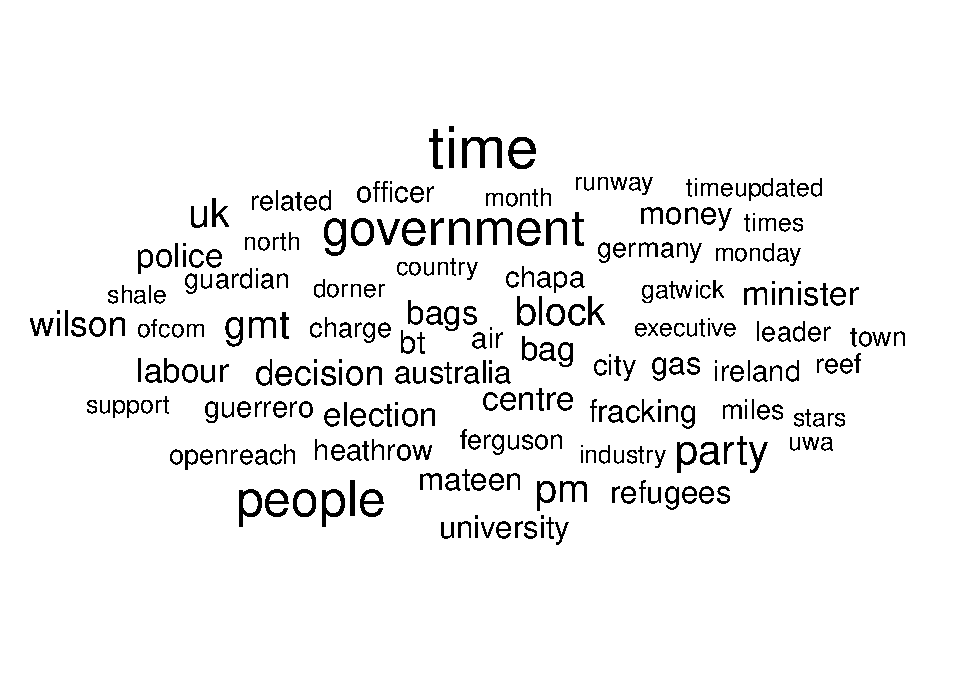
\includegraphics{2021_apis_for_social_scientists_a_collaborative_review_files/figure-latex/unnamed-chunk-14-1.pdf}
\caption{\label{fig:unnamed-chunk-14}Wordcloud of nouns found within guardian articles}
\end{figure}

\hypertarget{social-science-examples}{%
\section{Social science examples}\label{social-science-examples}}

\begin{itemize}
\tightlist
\item
  \emph{Are there social science research examples using the API?}
\end{itemize}

Text-as-data has become quite a common approach in the social sciences (see e.g., \citet{Grimmer2013-xe} for an overview). For the usage of Google's Natural Language API we however have the impression that it is relatively unknown in NLP and among social scientists. Hence, we want to emphasize the usefulness and importance the usage of Google's NLP API could have in many research projects.

However, if you are considering making use of it, keep two things in mind:

\begin{itemize}
\item
  some might interpret using the API as a ``blackbox'' approach (see \citet{Dobbrick2021-iz} for very recent developments of ``glass-box machine learning appraoches'' for text analysis) potentially standing in way of transparency and replication (two important criteria of good research?). However it is always possible to perform robustness and sensitivity analysis and to add the version of the API one was using.
\item
  depending on how large your corpus of text data, Google might charges you some money. However for up to 5,000 units (i.e., terms) the different variants of sentiment and syntax analysis are free. Check this overview by Google to learn about prices for more units \href{\%22https://cloud.google.com/natural-language/pricing\%22}{here}. Generally, also consider that if you are pursuing a CSS-related project in which the GCP Products would come in useful, there is the possibility to achieve Google Cloud Research credits (see \href{\%22https://edu.google.com/programs/credits/research/?modal_active=none\%22}{here}).
\end{itemize}

\hypertarget{google-translation-api}{%
\chapter{Google Translation API}\label{google-translation-api}}

Paul C. Bauer, Camille Landesvatter

\hypertarget{provided-servicesdata-1}{%
\section{Provided services/data}\label{provided-servicesdata-1}}

\begin{itemize}
\tightlist
\item
  \emph{What data/service is provided by the API?}
\end{itemize}

The API is provided by Google.

Google's Translation API translates texts into more than one hundred \href{\%22https://cloud.google.com/translate/docs/languages\%22}{languages}. Note that the approach via the API is a lot more refined than the \href{\%22https://translate.google.com/?hl=de\%22}{free version} on Googles' translation website and of course comes in very useful if text in large scale needs to be translated (possibly with longer and more complex content or syntax). For instance, you can choose to specify a certain model to further improve the translation (\href{\%22https://cloud.google.com/translate/docs/basic/translating-text\#translate_translate_text-python\%22}{Neural Machine Translation vs.~Phrase-Based Machine Translation}).

The API limits in three ways: characters per day, characters per 100 seconds, and API requests per 100 seconds. All can be set in the \href{\%22https://console.developers.google.com/apis/api/translate.googleapis.com/quotas\%22}{API manager} of your Google Cloud Project.

Consider that additionally to the Translation API which we demonstrate in this review, Google provides us with two further APIs for translation: AutoML Translation and the Advanced Translation API (see \href{\%22https://cloud.google.com/translate/?utm_source=google\&utm_medium=cpc\&utm_campaign=emea-de-all-de-dr-bkws-all-all-trial-e-gcp-1010042\&utm_content=text-ad-none-any-DEV_c-CRE_170514365277-ADGP_Hybrid\%20\%7C\%20BKWS\%20-\%20EXA\%20\%7C\%20Txt\%20~\%20AI\%20\%26\%20ML\%20~\%20Cloud\%20Translation\%23v3-KWID_43700053282385063-kwd-74703397964-userloc_9042003\&utm_term=KW_google\%20translator\%20api-NET_g-PLAC_\&gclid=CjwKCAjw_JuGBhBkEiwA1xmbRZOxg7QzGmhTHWseHFN_V0Al_Xlf8wZVBfX9EURtitWDbe2dLcTWIxoCjj0QAvD_BwE\&gclsrc=aw.ds\#section-4\%22}{here} for a short comparison).

\hypertarget{prerequesites-1}{%
\section{Prerequesites}\label{prerequesites-1}}

\begin{itemize}
\tightlist
\item
  \emph{What are the prerequisites to access the API (authentication)? }
\end{itemize}

To access and to use the API the following steps are necessary:

\begin{itemize}
\item
  Create a \href{\%22https://www.google.com/account/about/\%22}{google account} (if you do not already have one).
\item
  Using this google account login to the \href{\%22https://cloud.google.com/\%22}{google cloud platform} and create a Google Cloud Project.
\item
  Within this Google Cloud Project enable the Google Translation API.
\item
  For authentication you will need to create an API key (which you additionally should restrict to the Translation API). If however, you are planning to request the Natural Language API from outside a Google Cloud environment (e.g., R) you will be required to use a private (service account) key. This can be achieved by creating a service account which in turn will allow you to download your private key as a JSON file (we show an example below).
\end{itemize}

\hypertarget{simple-api-call-1}{%
\section{Simple API call}\label{simple-api-call-1}}

\begin{itemize}
\tightlist
\item
  \emph{What does a simple API call look like?}
\end{itemize}

Here we describe how a simple API call can be made from within the Google Cloud Platform environment via the Google Cloud Shell:

\begin{itemize}
\item
  To activate your Cloud Shell, inspect the upper right-hand corner of your Google Cloud Platform Console and click the icon called ``Activate Shell''. \href{\%22https://cloud.google.com/shell/\#how_do_i_get_started\%22}{Google Cloud Shell} is a command line environment running in the cloud.
\item
  Via the built-in Editor in Cloud Shell create a JSON file (call it for instance `request.json') with the text that you would like to perform analysis on. Consider that text can be uploaded in the request (shown below) or integrated with Cloud Storage. Supported types of your text are PLAIN\_TEXT (shown below) or HTML.
\end{itemize}

\begin{Shaded}
\begin{Highlighting}[]
\NormalTok{\{}
 \StringTok{"q"}\SpecialCharTok{:}\NormalTok{ [}\StringTok{"To administer medicine to animals is frequently a very difficult matter, and yet sometimes it’s necessary to do so"}\NormalTok{], }
\StringTok{"target"}\SpecialCharTok{:} \StringTok{"de"}
\NormalTok{\}}
\end{Highlighting}
\end{Shaded}

\begin{itemize}
\item
  For sending your data, pass a curl command to your Cloud Shell command line where you refer (via @) to your request.json file from the previous step.
\item
  Don't forget to insert your individual API key in the curl command (alternatively, you could define it beforehand via adding a global variable to your environment → see example in the API call for Googles' NLP API earlier in this document).
\end{itemize}

\begin{Shaded}
\begin{Highlighting}[]
\NormalTok{curl }\StringTok{"https://translation.googleapis.com/language/translate/v2?key=APIKEY"} \SpecialCharTok{{-}}\NormalTok{s }\SpecialCharTok{{-}}\NormalTok{X POST }\SpecialCharTok{{-}}\NormalTok{H }\StringTok{"Content{-}Type: application/json"} \SpecialCharTok{{-}{-}}\NormalTok{data}\SpecialCharTok{{-}}\NormalTok{binary }\SpecialCharTok{@}\NormalTok{request.json}
\end{Highlighting}
\end{Shaded}

\hypertarget{api-access-1}{%
\section{API access}\label{api-access-1}}

\begin{itemize}
\tightlist
\item
  \emph{How can we access the API from R (httr + other packages)?}
\end{itemize}

The following example makes use of the \href{\%22https://cran.r-project.org/web/packages/googleLanguageR/index.html\%22}{`googleLanguageR'} package from R which among other options (e.g., syntax analysis → see Chapter 2 of this review) allows calling the Cloud Translation API.

In this small example we demonstrate how to\ldots{}

\begin{itemize}
\item
  \ldots{} authenticate with your Google Cloud Account within R
\item
  \ldots{} translate an exemplary sentence
\end{itemize}

\emph{Step 1: Load package}

\begin{Shaded}
\begin{Highlighting}[]
\FunctionTok{library}\NormalTok{(googleLanguageR)}
\end{Highlighting}
\end{Shaded}

\emph{Step 2: Authentication}

\begin{Shaded}
\begin{Highlighting}[]
\FunctionTok{gl\_auth}\NormalTok{(}\StringTok{"./your{-}key.json"}\NormalTok{)}
\end{Highlighting}
\end{Shaded}

\emph{Step 3: Analysis - API call and Translation}

First, we create exemplary data. For demonstration purposes, we here again make use of the sentence from above. Of course, for your own project use a complete vector containing text data from within your data.

\begin{Shaded}
\begin{Highlighting}[]
\NormalTok{df\_original }\OtherTok{\textless{}{-}} \FunctionTok{data.frame}\NormalTok{(}\AttributeTok{text =} \StringTok{"To administer medicine to animals is frequently a very difficult matter, and yet sometimes it’s necessary to do so"}\NormalTok{)}

\NormalTok{df\_original}\SpecialCharTok{$}\NormalTok{text }\OtherTok{\textless{}{-}} \FunctionTok{as.character}\NormalTok{(df\_original}\SpecialCharTok{$}\NormalTok{text)}
\end{Highlighting}
\end{Shaded}

Next, using this data, call the API via the function `gl\_translate()' and importantly specify the target language (german in this example) within the `target' argument.

\begin{Shaded}
\begin{Highlighting}[]
\NormalTok{df\_translate }\OtherTok{\textless{}{-}} \FunctionTok{gl\_translate}\NormalTok{(df\_original}\SpecialCharTok{$}\NormalTok{text, }\AttributeTok{target =} \StringTok{"de"}\NormalTok{)}
\end{Highlighting}
\end{Shaded}

This API call eventually provides reuslts in a dataframe with three columns: translatedText ( → contains the translation), detectedSourceLangauge ( → contains a label for the original language being detected) and text ( → contains the original text).

Let's check the translation.

\begin{Shaded}
\begin{Highlighting}[]
\NormalTok{df\_translate}\SpecialCharTok{$}\NormalTok{translatedText}
\end{Highlighting}
\end{Shaded}

\emph{Tieren Medikamente zu verabreichen ist oft eine sehr schwierige Angelegenheit, und doch ist es manchmal notwendig}

\hypertarget{social-science-examples-1}{%
\section{Social science examples}\label{social-science-examples-1}}

\begin{itemize}
\tightlist
\item
  \emph{Are there social science research examples using the API?}
\end{itemize}

Searching on literature using Google Translation Services we found a study by \citet{Prates2018-fx} (\href{\%22https://arxiv.org/abs/1809.02208\%22}{Assessing gender bias in machine translation: a case study with Google Translate}).

We are not aware of any further research / publications that made explicit usage of Google's Translation API. However, we assume that the API (or at least Google's Free Translation Service) is involved in many research projects. Generally, we are convinced that making use of automated translation (as well as converting speech to text ( → example also in this review) eventually in combination with translation) can be of great advantage for all kinds of qualitative or mixed-methods research projects. For instance, automated translation could be very useful for easily and very reliably translating data from qualitative interviews or other (field) experiments or observational data (where data might be collected in a foreign language). Also consider the other way around where data is available in the principal language of the research project but some of the textual data has to be communicated and presented in (for instance) english language.

\hypertarget{crowdtangle-api}{%
\chapter{CrowdTangle API}\label{crowdtangle-api}}

Lion Behrens and Pirmin Stöckle

CrowdTangle is a public insights tool, whose main intent was to monitor what content overperformed in terms of interactions (likes, shares, etc.) on Facebook and other social media platforms. In 2016, CrowdTangle was acquired by Facebook that now provides the service.

\hypertarget{provided-servicesdata-2}{%
\section{Provided services/data}\label{provided-servicesdata-2}}

\begin{itemize}
\tightlist
\item
  \emph{What data/service is provided by the API?}
\end{itemize}

CrowdTangle allows users to systematically follow and analyze what is happening with public content on the social media platforms of Facebook, Twitter, Instagram and Reddit.
The data that can be assessed through the CrowdTangle API consists of any post that was made by a public page, group or verified public person who has ever acquired more than 110,000 likes since the year 2014 or has ever been added to the list of tracked public accounts by any active API user. If a new public page or group is added, data is pulled back from day one.

Data that is tracked:

\begin{itemize}
\tightlist
\item
  Content (the content of a post, including text, included links, links to included images or videos)
\item
  Interactions (count of likes, shares, comments, emoji-reactions)
\item
  Page Followers
\item
  Facebook Video Views
\item
  Benchmark scores of all metrics from the middle 50\% of posts in the same category (text, video) from the respective account
\end{itemize}

Data that is not tracked:

\begin{itemize}
\tightlist
\item
  Comments (while the number of comments is included, the content of the comments is not)
\item
  Demographical data
\item
  Page reach, traffic and clicks
\item
  Private posts and profiles
\item
  Ads only appear in the ad library (which is public), boosted content cannot differentiated from organic content
\end{itemize}

CrowdTangle's database is updated once every fifteen minutes and comes as time-series data which merges the content of a post on one of the included platforms (a text post, video, or image) alongside aggregate information on the post's views, likes and interactions.

When connecting to the user interface via the CrowdTangle website, the user can either manually set up a list of pages of interest whose data should be acquired. Alternatively, one can choose from an extensive number of pre-prepared lists covering a variety of topics, regions, or socially and politically relevant events such as inaugurations and elections. Data can be downloaded from the user interface as csv files or as json files via the API.

\hypertarget{prerequesites-2}{%
\section{Prerequesites}\label{prerequesites-2}}

\begin{itemize}
\tightlist
\item
  \emph{What are the prerequisites to access the API (authentication)? }
\end{itemize}

Full access to the CrowdTangle API is only given to Facebook partners who are in the business of publishing original content or fact-checkers as part of Facebook's Third-Party Fact-Checking program.
From 2019, the CrowdTangle API and user interface is also available for academics and researchers in specific fields. Currently, this prioritization includes research on one of the following fields: misinformation, elections, COVID-19 racial justice, well-being. To get access to CrowdTangle, a formal request has to be filed via an online form, asking for a short description of the research project and intended use of the data.

As a further restriction, CrowdTangle currently only allows academic staff, faculty and registered PhD students permission to obtain a CrowdTangle account. This does not include individuals enrolled as students at a university unless they are employed as research assistants. Also, certain access policies differ between academics and the private sector. Usage of CrowdTangle for research purposes does currently not provide access to any content posted on Reddit given that data is retrieved via the Application Programming Interface. Content from Reddit is open to every registered user only when navigating through the company's dynamic user interface that does not imply usage of any scripting language.
Finally, the CrowdTangle API requires researchers to log in using an existing Facebook account.
Overall, access to the API is quite restrictive, both because of the prioritization of certain research areas, and because the access request will be decided individually so that an immediate access is not possible. If access is granted, CrowdTangle provides quite extensive onboarding and training resources to use the API.

\emph{Replicability}

Access to CrowdTangle is gated and Facebook does not allow data from CrowdTangle to be published. So researchers can publish aggregate results from analyses on the data, but not the original data, which might be problematic for the replicability of research conducted with the API. A possible workaround is that you can pull ID numbers of posts in your dataset, which can then be used by anyone with a CrowdTangle API access to recreate your dataset.
CrowdTangle also provides some publicly available features such as a Link Checker Chrome Extension, allowing users to see how often a specific link has been shared on social media, and a curated public hub of Live displays, giving insight about specific topics on Facebook, Instagram and Reddit.

\hypertarget{simple-api-call-2}{%
\section{Simple API call}\label{simple-api-call-2}}

\begin{itemize}
\tightlist
\item
  \emph{What does a simple API call look like?}
\end{itemize}

All requests to the CrowdTangle API are made via GET to \url{https://api.crowdtangle.com/}.

In order to access data, users log in on the website with their Facebook account and acquire a personalized token. The CrowdTangle API expects the API token to be included in each query.
With one of these available endpoints, each of which comes with a set of specific parameters:

\begin{longtable}[]{@{}
  >{\raggedright\arraybackslash}p{(\columnwidth - 2\tabcolsep) * \real{0.50}}
  >{\raggedright\arraybackslash}p{(\columnwidth - 2\tabcolsep) * \real{0.50}}@{}}
\toprule
\endhead
GET /posts & Retrieve a set of posts for the given parameters. \\
GET /post & Retrieves a specific post. \\
GET /posts/search & Retrieve a set of posts for the given parameters and search terms. \\
GET /leaderboard & Retrieves leaderboard data for a certain list or set of accounts. \\
GET /links & Retrieve a set of posts matching a certain link. \\
GET /lists & Retrieve the lists, saved searches and saved post lists of the dashboard associated with the token sent in. \\
\bottomrule
\end{longtable}

\emph{A simple example: Which party or parties posted the 10 most successful Facebook posts this year?}

On the user interface, I created a list of the pages of all parties currently in the German Bundestag. We want to find out which party or parties posted the 10 most successful posts (i.e.~the posts with the most interactions) this year.

The respective API call looks like that:
\href{\%22https://api.crowdtangle.com/posts?token=token\&listIds=listIDs\&sortBy=total_interactions\&startDate=2021-01-01\&count=10\%22\%5D}{https://api.crowdtangle.com/posts?token=token\&listIds=listIDs\&sortBy=total\_interactions\&startDate=2021-01-01\&count=10}, where token is the personal API key, and listIDs is the ID of the list created with the user interface. Here, we sortBy total interactions with the startDate at the beginning of this year and the output restricted to count 10 posts.

\hypertarget{api-access-2}{%
\section{API access}\label{api-access-2}}

\begin{itemize}
\tightlist
\item
  \emph{How can we access the API from R (httr + other packages)?}
\end{itemize}

Instead of typing the API request into our browser, we can use the httr package's GET function to access the API from R.

\begin{Shaded}
\begin{Highlighting}[]
\CommentTok{\# Option 1: Accessing the API with base "httr" commands}
\FunctionTok{library}\NormalTok{(httr)}
 
\NormalTok{ct\_posts\_resp }\OtherTok{\textless{}{-}} \FunctionTok{GET}\NormalTok{(}\StringTok{"https://api.crowdtangle.com/posts"}\NormalTok{,}
    \AttributeTok{query=}\FunctionTok{list}\NormalTok{(}\AttributeTok{token =}\NormalTok{ token, }\CommentTok{\# API key has to be included in every query}
               \AttributeTok{listIds =}\NormalTok{ listIds, }\CommentTok{\# ID of the created list of pages or groups}
               \AttributeTok{sortBy =} \StringTok{"total\_interactions"}\NormalTok{,}
               \AttributeTok{startDate =} \StringTok{"2021{-}01{-}01"}\NormalTok{,}
               \AttributeTok{count =} \DecValTok{10}\NormalTok{))}
 
\NormalTok{ct\_posts\_list }\OtherTok{\textless{}{-}} \FunctionTok{content}\NormalTok{(ct\_posts\_resp)}
\FunctionTok{class}\NormalTok{(ct\_posts\_list) }\CommentTok{\# verify that the output is a list}
 
\CommentTok{\# List content}
\FunctionTok{str}\NormalTok{(ct\_posts\_list, }\AttributeTok{max.level =} \DecValTok{3}\NormalTok{) }\CommentTok{\# show structure \& limit levels}
 
\CommentTok{\# with some list operations we can get a dataframe with the account name and post date of the 10 posts with the most interactions in 2021 among the pages in the list}
\NormalTok{list\_part }\OtherTok{\textless{}{-}}\NormalTok{ rlist}\SpecialCharTok{::}\FunctionTok{list.select}\NormalTok{(ct\_posts\_list}\SpecialCharTok{$}\NormalTok{result}\SpecialCharTok{$}\NormalTok{posts, account}\SpecialCharTok{$}\NormalTok{name, date)}
\NormalTok{rlist}\SpecialCharTok{::}\FunctionTok{list.stack}\NormalTok{(list\_part)}
\end{Highlighting}
\end{Shaded}

Alternatively, we can use a wrapper function for R, which is provided by the RCrowdTangle package available on \href{\%22https://github.com/cbpuschmann/RCrowdTangle\%22}{github}. The package provides wrapper functions for the /posts, /posts/search, and /links endpoints. Conveniently, the wrapper function directly produces a dataframe as output, which is typically what we want to work with. As the example below shows, the wrapper function may not include the specific information we are looking for, however, as the example also shows, it is relatively straightforward to adapt the function on our own depending on the specific question at hand.
To download the package from github, we need to load the devtools package, and to use the wrapper function, we need dplyr and jsonlite.

\begin{Shaded}
\begin{Highlighting}[]
\CommentTok{\# Option 2: There is a wrapper function for R, which can be downloaded from github}

\FunctionTok{library}\NormalTok{(devtools) }\CommentTok{\# to download from github}
 
\FunctionTok{install\_github}\NormalTok{(}\StringTok{"cbpuschmann/RCrowdTangle"}\NormalTok{)}
\FunctionTok{library}\NormalTok{(RCrowdTangle)}
 
\CommentTok{\# The R wrapper relies on jsonlite and dplyr}
\FunctionTok{library}\NormalTok{(dplyr)}
\FunctionTok{library}\NormalTok{(jsonlite)}
 
\NormalTok{ct\_posts\_df }\OtherTok{\textless{}{-}} \FunctionTok{ct\_get\_posts}\NormalTok{(listIds, }\AttributeTok{startDate =} \StringTok{"2021{-}01{-}01"}\NormalTok{, }\AttributeTok{token =}\NormalTok{ token)}
 
\CommentTok{\#conveniently, the wrapper function directly produces a dataframe}
\FunctionTok{class}\NormalTok{(ct\_posts\_df)}
 
\CommentTok{\# to sort by total interactions we have to compute that figure because it is not part of the dataframe}
\NormalTok{ct\_posts\_df }\SpecialCharTok{\%\textgreater{}\%}
  \FunctionTok{mutate}\NormalTok{(}\AttributeTok{total\_interactions =}\NormalTok{ statistics.actual.likeCount}\SpecialCharTok{+}\NormalTok{statistics.actual.shareCount}\SpecialCharTok{+}\NormalTok{ statistics.actual.commentCount}\SpecialCharTok{+}\NormalTok{  statistics.actual.loveCount}\SpecialCharTok{+}\NormalTok{ statistics.actual.wowCount}\SpecialCharTok{+}\NormalTok{ statistics.actual.hahaCount}\SpecialCharTok{+}\NormalTok{ statistics.actual.sadCount}\SpecialCharTok{+}
\NormalTok{           statistics.actual.angryCount}\SpecialCharTok{+}\NormalTok{ statistics.actual.thankfulCount}\SpecialCharTok{+}\NormalTok{ statistics.actual.careCount) }\SpecialCharTok{\%\textgreater{}\%}
  \FunctionTok{arrange}\NormalTok{(}\FunctionTok{desc}\NormalTok{(total\_interactions)) }\SpecialCharTok{\%\textgreater{}\%}
  \FunctionTok{select}\NormalTok{(account.name, date) }\SpecialCharTok{\%\textgreater{}\%}
  \FunctionTok{head}\NormalTok{(}\AttributeTok{n=}\DecValTok{10}\NormalTok{)}
 
\CommentTok{\# alternatively, we can adapt the wrapper function by ourselves to include the option to sort by total interactions}
\NormalTok{ct\_get\_posts }\OtherTok{\textless{}{-}} \ControlFlowTok{function}\NormalTok{(}\AttributeTok{x =} \StringTok{""}\NormalTok{, }\AttributeTok{searchTerm =} \StringTok{""}\NormalTok{, }\AttributeTok{language =} \StringTok{""}\NormalTok{, }\AttributeTok{types=} \StringTok{""}\NormalTok{, }\AttributeTok{minInteractions =} \DecValTok{0}\NormalTok{, }\AttributeTok{sortBy =} \StringTok{""}\NormalTok{, }\AttributeTok{count =} \DecValTok{100}\NormalTok{, }\AttributeTok{startDate =} \StringTok{""}\NormalTok{, }\AttributeTok{endDate =} \StringTok{""}\NormalTok{, }\AttributeTok{token =} \StringTok{""}\NormalTok{)}
\NormalTok{\{}
\NormalTok{  endpoint.posts }\OtherTok{\textless{}{-}} \StringTok{"https://api.crowdtangle.com/posts"}
\NormalTok{  query.string }\OtherTok{\textless{}{-}} \FunctionTok{paste0}\NormalTok{(endpoint.posts, }\StringTok{"?listIds="}\NormalTok{, x, }\StringTok{"\&searchTerm="}\NormalTok{, searchTerm, }\StringTok{"\&language="}\NormalTok{, language, }\StringTok{"\&types="}\NormalTok{, types, }\StringTok{"\&minInteractions="}\NormalTok{, minInteractions, }\StringTok{"\&sortBy="}\NormalTok{, sortBy, }\StringTok{"\&count="}\NormalTok{, count, }\StringTok{"\&startDate="}\NormalTok{, startDate, }\StringTok{"\&endDate="}\NormalTok{, endDate, }\StringTok{"\&token="}\NormalTok{, token)}
\NormalTok{  response.json }\OtherTok{\textless{}{-}} \FunctionTok{try}\NormalTok{(}\FunctionTok{fromJSON}\NormalTok{(query.string), }\AttributeTok{silent =} \ConstantTok{TRUE}\NormalTok{)}
\NormalTok{  status }\OtherTok{\textless{}{-}}\NormalTok{ response.json}\SpecialCharTok{$}\NormalTok{status}
\NormalTok{  nextpage }\OtherTok{\textless{}{-}}\NormalTok{ response.json}\SpecialCharTok{$}\NormalTok{result}\SpecialCharTok{$}\NormalTok{pagination}\SpecialCharTok{$}\NormalTok{nextPage}
\NormalTok{  posts }\OtherTok{\textless{}{-}}\NormalTok{ response.json}\SpecialCharTok{$}\NormalTok{result}\SpecialCharTok{$}\NormalTok{posts }\SpecialCharTok{\%\textgreater{}\%} \FunctionTok{select}\NormalTok{(}\SpecialCharTok{{-}}\NormalTok{expandedLinks, }\SpecialCharTok{{-}}\NormalTok{media) }\SpecialCharTok{\%\textgreater{}\%} \FunctionTok{flatten}\NormalTok{()}
  \FunctionTok{return}\NormalTok{(posts)}
\NormalTok{\}}
 
\NormalTok{ct\_posts\_df }\OtherTok{\textless{}{-}} \FunctionTok{ct\_get\_posts}\NormalTok{(listIds, }\AttributeTok{sortBy =} \StringTok{"total\_interactions"}\NormalTok{, }\AttributeTok{startDate =} \StringTok{"2021{-}01{-}01"}\NormalTok{, }\AttributeTok{token =}\NormalTok{ token)}
 
\NormalTok{ct\_posts\_df }\SpecialCharTok{\%\textgreater{}\%}
  \FunctionTok{select}\NormalTok{(account.name, date) }\SpecialCharTok{\%\textgreater{}\%}
  \FunctionTok{head}\NormalTok{(}\AttributeTok{n=}\DecValTok{10}\NormalTok{)}
\end{Highlighting}
\end{Shaded}

\hypertarget{social-science-examples-2}{%
\section{Social science examples}\label{social-science-examples-2}}

\begin{itemize}
\tightlist
\item
  \emph{Are there social science research examples using the API?}
\end{itemize}

A common use case is to track the spread of specific links containing misinformation, e.g.~conspiracy around the connection of COVID-19 and 5G (\citet{Bruns2020-pl}).
\citet{Berriche2020-dt} provide an in-depth analysis of a specific page involved in online health misinformation and investigate factors driving interactions with the respective posts. They find that users mainly interact to foster social relations, not to spread misinformation.
CrowdTangle has also been used to study changes in the framing of vaccine refusal by analyzing content of posts by pages opposing vaccinations over time (\citet{Broniatowski2020-rh}).
Another approach is to monitor political communication of political actors, specifically in the run-up to elections. \citet{Larsson2020-iu} investigates a one-month period before the 2018 Swedish election and finds that right-wing political actors are more successful than mainstream actors in engaging their Facebook followers, often using sensational rhetoric and hate-mongering.

\hypertarget{google-places-api}{%
\chapter{Google Places API}\label{google-places-api}}

Lukas Isermann and Clara Husson

\hypertarget{provided-servicesdata-3}{%
\section{Provided services/data}\label{provided-servicesdata-3}}

\begin{itemize}
\tightlist
\item
  \emph{What data/service is provided by the API?}
\end{itemize}

The following five requests are available: Place Search, Place Details, Place Photos, Place Autocomplete and Query Autocomplete. Place Search returns a list of places along with summary information about each place based on a user's location (by proximity) or search string. Once you find a place\_id from a Place Search, you can request more details about a particular place by doing a Place Details request. A Place Details request returns more detailed information about the indicated place such as its complete address, phone number, user rating and reviews. Place Photos provides access to the millions of place-related photos stored in Google's Place database. When you get place information using a Place Details request, photo references will be returned for relevant photographic content. Find Place, Nearby Search, and Text Search requests also return a single photo reference per place, when relevant. Place Autocomplete automatically fills in the name and/or address of a place as users type. Query Autocomplete service provides a query prediction for text-based geographic searches, by returning suggested queries as you type.

\textbf{Note:} You can display Places API results on a Google Map, or without a map but it is prohibited to use Places API data on a map that is not a Google map.

\hypertarget{prerequesites-3}{%
\section{Prerequesites}\label{prerequesites-3}}

\begin{itemize}
\tightlist
\item
  \emph{What are the prerequisites to access the API (authentication)? }
\end{itemize}

The prerequisites to access Google Places API are a Google Cloud project (to create it you need a Google account to log into the Google Cloud Platform) and an API Key. Before creating your API Key, don't forget to enable Places API! To create your API key, go the APIs \& Services \textgreater{} Credentials \textgreater{} API key page.

\hypertarget{simple-api-call-3}{%
\section{Simple API call}\label{simple-api-call-3}}

\begin{itemize}
\tightlist
\item
  \emph{What does a simple API call look like?}
\end{itemize}

The API provides different searches and services that can be accessed via HTTP Urls. These Urls requests all take the same general form and pattern:

\url{https://maps.googleapis.com/maps/api/place/service/output?parameters}

Here, service can take the inputs findplacefromtext for find place requests, nearbysearch to look for nearby places, details for a request of place details and more. output may take the value json or xml, dependent on the requested output format.

Furthermore, certain parameters are required for all requests. Most importantly, every request must entail a key parameter, indicating the API key. Second, all search places requests take an input parameter that identifies the search target and an inputtype parameter that identifies the type of input given in the input parameter. For place requests, the inputtype parameter can take the values textquery and phonenumber.

Nearby requests take a location parameter setting longitude and latitude of the requested place as well as a radius parameter. Detail request, however, take a mandatory parameter place\_id, which indicates the place for which the details are requested.

Additionally, different optional parameters can be used. These entail a language parameter, a fields parameter indicating the types of place data to return and more.

An examples for an API request for pizza places in Mannheim can look like this:

\url{https://maps.googleapis.com/maps/api/place/textsearch/xml?query=pizza\&location=49.487459,8.466039\&radius=5000\&key=YOUR_API_KEY}

\hypertarget{api-access-3}{%
\section{API access}\label{api-access-3}}

\begin{itemize}
\tightlist
\item
  \emph{How can we access the API from R (httr + other packages)?}
\end{itemize}

Instead of typing the API request into our browser, we can use the httr package's GET function to access the API from R.

\begin{Shaded}
\begin{Highlighting}[]
\CommentTok{\# Option 1: Accessing the API with base "httr" commands}
\FunctionTok{library}\NormalTok{(httr)}

\NormalTok{key }\OtherTok{\textless{}{-}} \StringTok{"YOURAPIKEY"}

\NormalTok{res}\OtherTok{\textless{}{-}}\FunctionTok{GET}\NormalTok{(}\StringTok{"https://maps.googleapis.com/maps/api/place/textsearch/json?"}\NormalTok{, }\AttributeTok{query =} \FunctionTok{list}\NormalTok{(}
           \AttributeTok{query =} \StringTok{"pizza"}\NormalTok{,}
           \AttributeTok{location =} \StringTok{"49.487459,8.466039"}\NormalTok{,}
           \AttributeTok{radius =} \DecValTok{5000}\NormalTok{,}
           \AttributeTok{key =}\NormalTok{ key}
\NormalTok{         ))}
\end{Highlighting}
\end{Shaded}

Alternatively, we can use a wrapper function for R provided by the R-Package googleway.

\emph{Authentication}

\begin{Shaded}
\begin{Highlighting}[]
\NormalTok{key }\OtherTok{\textless{}{-}} \StringTok{"YOURAPIKEY"}
\FunctionTok{set\_key}\NormalTok{(key)}
\end{Highlighting}
\end{Shaded}

\emph{API call}

\begin{Shaded}
\begin{Highlighting}[]
\CommentTok{\# Option 2: Accessing the API with googleway}

\FunctionTok{library}\NormalTok{(ggplot2)}
\FunctionTok{library}\NormalTok{(tidyverse)}
\FunctionTok{library}\NormalTok{(googleway)}

\CommentTok{\# Request \textquotesingle{}Mannheim\textquotesingle{} to get latitude and longitude information}
\NormalTok{location }\OtherTok{\textless{}{-}}\NormalTok{ googleway}\SpecialCharTok{::}\FunctionTok{google\_places}\NormalTok{(}\StringTok{"Mannheim"}\NormalTok{)}


\CommentTok{\# Save latitude and longitude information in vector}
\NormalTok{location }\OtherTok{\textless{}{-}}\NormalTok{ location}\SpecialCharTok{$}\NormalTok{results}\SpecialCharTok{$}\NormalTok{geometry}
\NormalTok{location }\OtherTok{\textless{}{-}} \FunctionTok{c}\NormalTok{(location}\SpecialCharTok{$}\NormalTok{location}\SpecialCharTok{$}\NormalTok{lat, location}\SpecialCharTok{$}\NormalTok{location}\SpecialCharTok{$}\NormalTok{lng)}


\CommentTok{\# Plot places to google map}
\FunctionTok{library}\NormalTok{(mapsapi)}
\CommentTok{\# for this you will also need to activate the "maps static API"}
\NormalTok{r }\OtherTok{=}\NormalTok{ mapsapi}\SpecialCharTok{::}\FunctionTok{mp\_map}\NormalTok{(}\AttributeTok{center =}\NormalTok{ (}\StringTok{"49.48746,8.466039"}\NormalTok{), }\AttributeTok{zoom =} \DecValTok{14}\NormalTok{, }\AttributeTok{key =}\NormalTok{ key, }\AttributeTok{quiet =} \ConstantTok{TRUE}\NormalTok{)}
\FunctionTok{library}\NormalTok{(stars)}
\FunctionTok{plot}\NormalTok{(r)}
\end{Highlighting}
\end{Shaded}

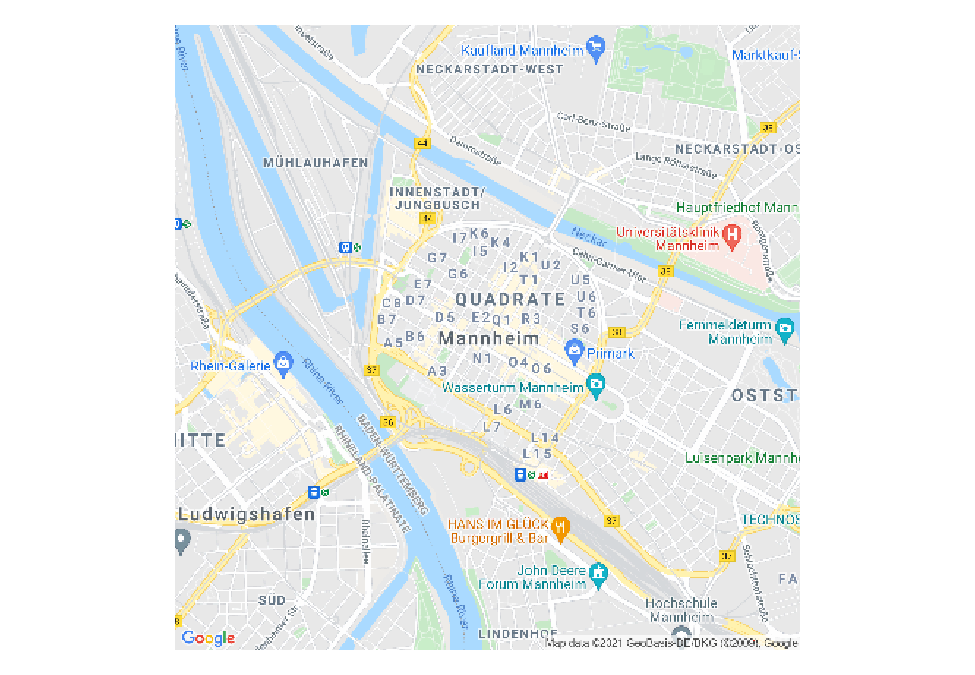
\includegraphics{2021_apis_for_social_scientists_a_collaborative_review_files/figure-latex/unnamed-chunk-28-1.pdf}

\begin{Shaded}
\begin{Highlighting}[]
\CommentTok{\# Google places request with googleway}
\NormalTok{pizza }\OtherTok{\textless{}{-}} \FunctionTok{google\_places}\NormalTok{(}\StringTok{"Pizza"}\NormalTok{, }\AttributeTok{location =}\NormalTok{ location, }\AttributeTok{radius =} \DecValTok{5000}\NormalTok{, }\AttributeTok{place\_type =} \StringTok{"food"}\NormalTok{)}

\CommentTok{\# Plot rankings as barplot}
\NormalTok{pizza}\SpecialCharTok{$}\NormalTok{results }\SpecialCharTok{\%\textgreater{}\%}
  \FunctionTok{ggplot}\NormalTok{() }\SpecialCharTok{+}
  \FunctionTok{geom\_col}\NormalTok{(}\FunctionTok{aes}\NormalTok{(}\AttributeTok{x =} \FunctionTok{reorder}\NormalTok{(name, rating), }\AttributeTok{y =}\NormalTok{ rating)) }\SpecialCharTok{+}
  \FunctionTok{geom\_text}\NormalTok{(}\FunctionTok{aes}\NormalTok{(}\AttributeTok{x =} \FunctionTok{reorder}\NormalTok{(name, rating), }\AttributeTok{y =}\NormalTok{ rating),}
                \AttributeTok{label =} \FunctionTok{paste0}\NormalTok{(pizza}\SpecialCharTok{$}\NormalTok{results}\SpecialCharTok{$}\NormalTok{user\_ratings\_total, }\StringTok{" }\SpecialCharTok{\textbackslash{}n}\StringTok{ ratings"}\NormalTok{), }\AttributeTok{size =} \DecValTok{2}\NormalTok{) }\SpecialCharTok{+}
  \FunctionTok{ylab}\NormalTok{(}\StringTok{"Average Rating"}\NormalTok{)}\SpecialCharTok{+}
  \FunctionTok{xlab}\NormalTok{(}\StringTok{""}\NormalTok{) }\SpecialCharTok{+}
  \FunctionTok{ggtitle}\NormalTok{(}\StringTok{"Pizza Places in Mannheim by Rating"}\NormalTok{) }\SpecialCharTok{+}
  \FunctionTok{theme\_minimal}\NormalTok{() }\SpecialCharTok{+}
  \FunctionTok{theme}\NormalTok{(}
    \AttributeTok{axis.text.x =} \FunctionTok{element\_text}\NormalTok{(}\AttributeTok{angle =} \DecValTok{90}\NormalTok{, }\AttributeTok{size =} \DecValTok{8}\NormalTok{, }\AttributeTok{hjust=}\FloatTok{0.95}\NormalTok{,}\AttributeTok{vjust=}\FloatTok{0.2}\NormalTok{))}
\end{Highlighting}
\end{Shaded}

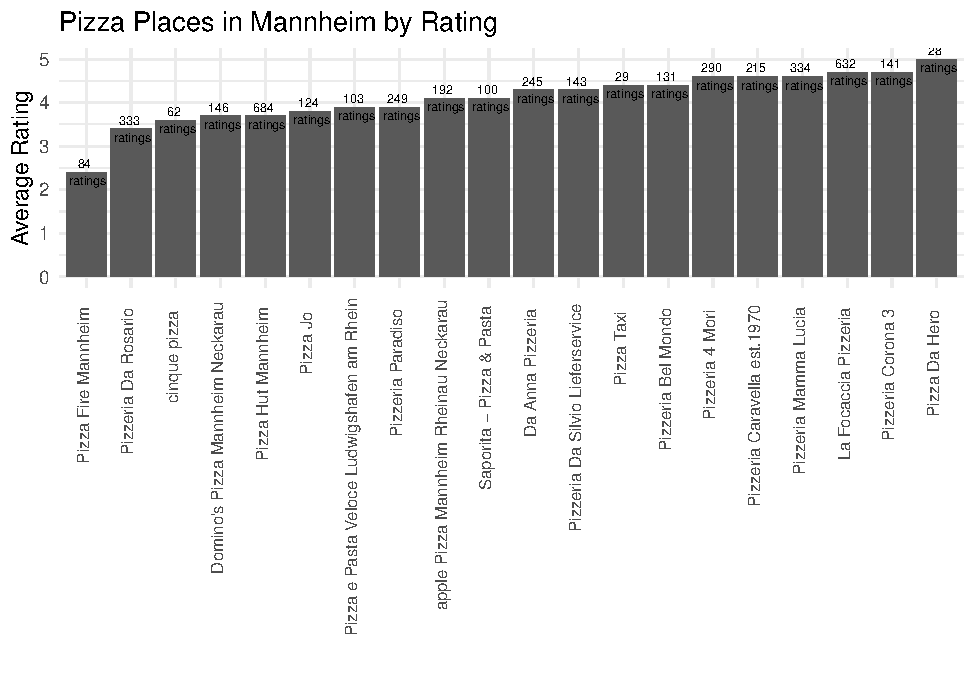
\includegraphics{2021_apis_for_social_scientists_a_collaborative_review_files/figure-latex/unnamed-chunk-29-1.pdf}

\begin{Shaded}
\begin{Highlighting}[]
\CommentTok{\# Plot pizza places to google map}
\CommentTok{\#important: in order to display the map correctly, you will also have to enable the Maps JavaScript API on GCP}
\CommentTok{\# unfortunately we can not display an intercative card in this document, but check out the below code in your own rmd{-}file! }

\NormalTok{map}\OtherTok{\textless{}{-}}\NormalTok{googleway}\SpecialCharTok{::}\FunctionTok{google\_map}\NormalTok{(}\AttributeTok{location =}\NormalTok{ location)}
\NormalTok{googleway}\SpecialCharTok{::}\FunctionTok{add\_markers}\NormalTok{(map, }\AttributeTok{data =}\NormalTok{ pizza}\SpecialCharTok{$}\NormalTok{results}\SpecialCharTok{$}\NormalTok{geometry}\SpecialCharTok{$}\NormalTok{location)}
\end{Highlighting}
\end{Shaded}

\hypertarget{social-science-examples-3}{%
\section{Social science examples}\label{social-science-examples-3}}

\begin{itemize}
\tightlist
\item
  \emph{Are there social science research examples using the API?}
\end{itemize}

In his study ``Using Google places data to analyze changes in mobility during the COVID-19 pandemic'', \citet{Konrad2020-rl} looked at the ``popular times'' data provided by Google Places to measure the effect of social distancing effort on mobility.

\hypertarget{google-speech-to-text-api}{%
\chapter{Google Speech-to-Text API}\label{google-speech-to-text-api}}

Camille Landesvatter

\hypertarget{provided-servicesdata-4}{%
\section{Provided services/data}\label{provided-servicesdata-4}}

\begin{itemize}
\tightlist
\item
  \emph{What data/service is provided by the API?}
\end{itemize}

Google's Speech-to-Text API allows you to convert audio files to text by applying powerful neural network models. Audio content can be transcribed in real time and of course (and possibly of higher relevance for social science research) from stored files.

The API currently recognizes more than 125 \href{\%22https://cloud.google.com/speech-to-text/docs/languages\%22}{languages}. It supports multiple audio formats, and audio files can either be transcribed directly (if the content does not exceed 60 seconds) or perform asynchronous requests for audio files longer than 60 seconds.

A demo of the API that allows you to record text via your microphone (or to upload an audio file) and explore the transcript can be found \href{\%22https://cloud.google.com/speech-to-text\#section-2\%22}{here}.

Also consider that there is a \href{\%22https://cloud.google.com/text-to-speech\%22}{Text-to-Speech API} - simply performing operations the other way around - offered by Google.

\hypertarget{prerequesites-4}{%
\section{Prerequesites}\label{prerequesites-4}}

\begin{itemize}
\tightlist
\item
  \emph{What are the prerequisites to access the API (authentication)? }
\end{itemize}

To access and to use the API the following steps are necessary:

\begin{itemize}
\item
  Create a \href{\%22https://www.google.com/account/about/\%22}{google account} (if you do not already have one).
\item
  With this google account login to the \href{\%22https://cloud.google.com/\%22}{google cloud platform} and create a Google Cloud Project.
\item
  Within this Google Cloud Project enable the Google Speech-to-text API.
\item
  For authentication you will need to create an API key (which you additionally should restrict to the Translation API). If however, you are planning to request the Natural Language API from outside a Google Cloud environment (e.g., R) you will be required to use a private (service account) key. This can be achieved by creating a service account which in turn will allow you to download your private key as a JSON file (we show an example below).
\end{itemize}

\hypertarget{simple-api-call-4}{%
\section{Simple API call}\label{simple-api-call-4}}

\begin{itemize}
\tightlist
\item
  \emph{What does a simple API call look like?}
\end{itemize}

\emph{Note.} For both Google's Translation API as well as Google's Natural-Language API, in this review we demonstrate an example for a simple API call via the Google Cloud Shell. In principle (and in a very similar procedure) this can be achieved for the Speech-to-Text API. However, your audio file will need some pre-processing. Audio data (such as our exemplary file in wav-format) is binary data. To make your REST request (via the Google Cloud Shell) however JSON is used. JSON eventually does not support binary data which is why you will have to transform your binary audio file into text using \href{\%22https://en.wikipedia.org/wiki/Base64\%22}{Base64} encoding (also refer to this \href{\%22https://cloud.google.com/speech-to-text/docs/base64-encoding\#linux\%22}{documentation} from the Google Website for more information). If you enter audio data which is not Base64 encoded, the Google Cloud Shell will give you an error 400 stating that Base64 decoding failed for your (wav-)file. Nevertheless, in the box below we will provide the basic structure of the request.

\begin{itemize}
\item
  To activate your Cloud Shell, inspect the upper right-hand corner of your Google Cloud Platform Console and click the icon called ``Activate Shell''. \href{\%22https://cloud.google.com/shell/\#how_do_i_get_started\%22}{Google Cloud Shell} is a command line environment running in the cloud.
\item
  Via the built-in Editor in Cloud Shell create a JSON file (call it for instance `request.json'). You can either upload your audio file directly via the Google Cloud Shell (search for the three-dotted ``More'' menu in the Shell and select ``Upload file''), alternatively audio content can be integrated with Cloud Storage.
\item
  The wav.file we uploaded for this example is an exemplary wav.file that comes along with the \href{\%22https://cran.r-project.org/web/packages/googleLanguageR/index.html\%22}{`googleLanguageR' R package}.
\end{itemize}

\begin{Shaded}
\begin{Highlighting}[]
\NormalTok{\{}
  \StringTok{"audio"}\SpecialCharTok{:}\NormalTok{ \{}
    \StringTok{"content"}\SpecialCharTok{:} \StringTok{"woman1\_wb"}
\NormalTok{  \},}
  \StringTok{"config"}\SpecialCharTok{:}\NormalTok{ \{}
    \StringTok{"enableAutomaticPunctuation"}\SpecialCharTok{:}\NormalTok{ true,}
    \StringTok{"encoding"}\SpecialCharTok{:} \StringTok{"LINEAR16"}\NormalTok{,}
    \StringTok{"languageCode"}\SpecialCharTok{:} \StringTok{"en{-}US"}\NormalTok{,}
    \StringTok{"model"}\SpecialCharTok{:} \StringTok{"default"}
\NormalTok{  \}}
\NormalTok{\}}
\end{Highlighting}
\end{Shaded}

\begin{itemize}
\item
  For sending your data, pass a curl command to your Cloud Shell command line where you refer (via @) to your request.json file from the previous step.
\item
  Don't forget to insert your individual API key (alternatively, you could define it beforehand via a variable in your environment -\textgreater{} see example in the API call for Google's NLP API later in this document).
\end{itemize}

\begin{Shaded}
\begin{Highlighting}[]
\NormalTok{curl }\StringTok{"https://speech.googleapis.com/v1p1beta1/speech:recognize?key=APIKEY"} \SpecialCharTok{{-}}\NormalTok{s }\SpecialCharTok{{-}}\NormalTok{X POST }\SpecialCharTok{{-}}\NormalTok{H }\StringTok{"Content{-}Type: application/json"} \SpecialCharTok{{-}{-}}\NormalTok{data}\SpecialCharTok{{-}}\NormalTok{binary }\SpecialCharTok{@}\NormalTok{request.json}
\end{Highlighting}
\end{Shaded}

\hypertarget{api-access-4}{%
\section{API access}\label{api-access-4}}

\begin{itemize}
\tightlist
\item
  \emph{How can we access the API from R (httr + other packages)?}
\end{itemize}

Example using R-Package \href{\%22https://cran.r-project.org/web/packages/googleLanguageR/index.html\%22}{`googleLanguageR'}

In this small example we demonstrate how to..

*.. authenticate with your Google Cloud Account within R

*.. how to import an exemplary audiofile from the ``GoogleLanguageR'' package

*.. how to transcribe this audio file and calculate a confidence score

For the usage of further arguments, also read the \texttt{gl\_speech()} \href{\%22https://cran.r-project.org/web/packages/googleLanguageR/googleLanguageR.pdf\%22}{documentation} and \href{\%22https://cran.r-project.org/web/packages/googleLanguageR/vignettes/speech.html\%22}{this} vignette.

\emph{1. Load packages}

\begin{Shaded}
\begin{Highlighting}[]
\FunctionTok{library}\NormalTok{(tidyverse)}
\FunctionTok{library}\NormalTok{(googleLanguageR)}
\end{Highlighting}
\end{Shaded}

\emph{Step 2: Authentication}

\begin{Shaded}
\begin{Highlighting}[]
\FunctionTok{gl\_auth}\NormalTok{(}\StringTok{"./your{-}key.json"}\NormalTok{)}
\end{Highlighting}
\end{Shaded}

\emph{Step 3: Analysis}

We will now get a sample source file which comes along with the \texttt{googleLanuageR} package. The transcript of this file is: ``To administer medicine to animals is frequently a very difficult matter, and yet sometimes it's necessary to do so'' - which according to \citet{Edmondson2017-pv} (one of the authors of the \href{\%22https://cran.r-project.org/web/packages/googleLanguageR/index.html\%22}{`googleLanguageR' R package}) is a fairly difficult sentence for computers to parse.

\begin{Shaded}
\begin{Highlighting}[]
\NormalTok{test\_audio }\OtherTok{\textless{}{-}} \FunctionTok{system.file}\NormalTok{(}\StringTok{"woman1\_wb.wav"}\NormalTok{, }\AttributeTok{package =} \StringTok{"googleLanguageR"}\NormalTok{)}
\end{Highlighting}
\end{Shaded}

We can now call the API via the function \texttt{gl\_speech()}. Here you will have to specify the quantity of interest, namely the \texttt{audio\_source} (this can either be a local file or a Google Cloud Storage URI) as well as the \texttt{languageCode} (language spoken in your audio file).

\begin{Shaded}
\begin{Highlighting}[]
\NormalTok{audio\_data }\OtherTok{\textless{}{-}} \FunctionTok{gl\_speech}\NormalTok{(}\AttributeTok{audio\_source=}\NormalTok{test\_audio, }\AttributeTok{languageCode =} \StringTok{"en{-}GB"}\NormalTok{)}
\end{Highlighting}
\end{Shaded}

The result is a list containing two dataframes: \texttt{transcript} and \texttt{timings}.

\begin{Shaded}
\begin{Highlighting}[]
\FunctionTok{dimnames}\NormalTok{(audio\_data}\SpecialCharTok{$}\NormalTok{transcript)}
\end{Highlighting}
\end{Shaded}

\begin{verbatim}
## [[1]]
## [1] "1"
## 
## [[2]]
## [1] "transcript"   "confidence"   "languageCode" "channelTag"
\end{verbatim}

The \texttt{timings} dataframe stores timestamps telling us when each specific term was recognised. The \texttt{transcript} dataframe importantly provides the transcript as well as a confidence score. We can see that the transcript misses one term (``a'') and indicates its confidence with a score close to 1.0.

\begin{Shaded}
\begin{Highlighting}[]
\NormalTok{audio\_data}\SpecialCharTok{$}\NormalTok{transcript}\SpecialCharTok{$}\NormalTok{transcript}
\end{Highlighting}
\end{Shaded}

\emph{to administer medicine to animals is frequently very difficult matter and yet sometimes it's necessary to do so}

\begin{Shaded}
\begin{Highlighting}[]
\NormalTok{audio\_data}\SpecialCharTok{$}\NormalTok{transcript}\SpecialCharTok{$}\NormalTok{confidence }\CommentTok{\#0.92}
\end{Highlighting}
\end{Shaded}

\begin{verbatim}
## [1] "0.9151855"
\end{verbatim}

\hypertarget{social-science-examples-4}{%
\section{Social science examples}\label{social-science-examples-4}}

\begin{itemize}
\tightlist
\item
  \emph{Are there social science research examples using the API?}
\end{itemize}

Similar to our note on social science research examples for Google's Translation API, we are not aware of research that made explicit usage of Google's Speech-to-text API.
However, and especially in combination with the Translation API, we are convinced that speech-to-text conversion can be of great advantage for all kinds of qualitative or mixed-methods research projects.

\hypertarget{instagram-graph-api}{%
\chapter{Instagram Graph API}\label{instagram-graph-api}}

Philipp Kadel

\hypertarget{provided-servicesdata-5}{%
\section{Provided services/data}\label{provided-servicesdata-5}}

\begin{itemize}
\tightlist
\item
  \emph{What data/service is provided by the API?}
\end{itemize}

The Instagram Graph API is provided by Facebook. There are two main APIs for Instagram, the Instagram Basic Display API and the \href{\%22https://developers.facebook.com/docs/instagram-api?locale=en_US\%22}{Instagram Graph API}. The latter is described in the following.

The API can be used to get and manage published photos, videos, and stories as well as getting basic data about other Instagram Business users and Creators. It is also possible to moderate comments and their replies and to measure media and profile interaction. Photos and videos can be published directly from the API. It can also be used to discover hashtagged media and mentions.

For photos and videos different metrics can be obtained:

\begin{itemize}
\tightlist
\item
  engagement -- Total number of likes and comments on the media object.
\item
  Impressions -- Total number of times the media object has been seen.
\item
  Reach -- Total number of unique accounts that have seen the media object.
\item
  Saved -- Total number of unique accounts that have saved the media object.
\item
  Video\_views -- (Videos only) Total number of times the video has been seen. Returns 0 for videos in carousel albums.
\end{itemize}

Likewise, there are several metrics about stories that are provided by the API:

\begin{itemize}
\tightlist
\item
  Exits -- Number of times someone exited the story.
\item
  Impressions -- Total number of times the story has been seen.
\item
  Reach -- Total number of unique accounts that have seen the story.
\item
  Replies -- Total number of replies to the story.
\item
  Taps\_forward -- Total number of taps to see this story's next photo or video.
\end{itemize}

\hypertarget{prerequesites-5}{%
\section{Prerequesites}\label{prerequesites-5}}

\begin{itemize}
\tightlist
\item
  \emph{What are the prerequisites to access the API (authentication)? }
\end{itemize}

For most endpoints you need an Instagram Business Account, a Facebook Page that is connected to that account, a Facebook Developer Account and a Facebook App with Basic settings configured. Facebook provides a tutorial for setting this up \href{\%22https://developers.facebook.com/docs/instagram-api/getting-started\%22}{here}.

\hypertarget{simple-api-call-5}{%
\section{Simple API call}\label{simple-api-call-5}}

\begin{itemize}
\tightlist
\item
  \emph{What does a simple API call look like?}
\end{itemize}

Below you can find expamples of simple API calls for the Instagram Graph API.

Get Fields and Edges on an IG Media. Fields can be e.g., ``caption'', ``comments\_count'', ``like\_count'', or ``timestamp''.

\begin{itemize}
\tightlist
\item
  GET (``\url{https://graph.facebook.com/v10.0/\%7Big-media-id\%7D} ?fields=\{fields\} \&access\_token=\{access-token\}'')
\end{itemize}

Example:

\begin{Shaded}
\begin{Highlighting}[]
\FunctionTok{GET}\NormalTok{ (“https}\SpecialCharTok{:}\ErrorTok{//}\NormalTok{graph.facebook.com}\SpecialCharTok{/}\NormalTok{v10}\FloatTok{.0}\SpecialCharTok{/}\DecValTok{17895695668004550}
\NormalTok{      ?}\AttributeTok{fields=}\NormalTok{id,media\_type,media\_url,owner,}
\NormalTok{      timestamp}\SpecialCharTok{\&}\AttributeTok{access\_token=}\NormalTok{IGQVJ...”)}
\end{Highlighting}
\end{Shaded}

Response:

\begin{Shaded}
\begin{Highlighting}[]
\NormalTok{\{}
  \StringTok{"id"}\SpecialCharTok{:} \StringTok{"17895695668004550"}\NormalTok{,}
  \StringTok{"media\_type"}\SpecialCharTok{:} \StringTok{"IMAGE"}\NormalTok{,}
  \StringTok{"media\_url"}\SpecialCharTok{:} \StringTok{"https://fb{-}s{-}b{-}a.akamaihd.net/h{-}ak{-}fbx/t51.2885{-}9/21227247\_1640962412602631\_3222510491855224832\_n.jpg?\_nc\_log=1"}\NormalTok{,}
  \StringTok{"owner"}\SpecialCharTok{:}\NormalTok{ \{}
    \StringTok{"id"}\SpecialCharTok{:} \StringTok{"17841405822304914"}
\NormalTok{  \},}
  \StringTok{"timestamp"}\SpecialCharTok{:} \StringTok{"2017{-}08{-}31T18:10:00+0000"}
\end{Highlighting}
\end{Shaded}

Return Fields and Edges on an IG Hashtag. Field can be the name of the hashtag without the ``\#'' symbol or a hashtag ID.

\begin{itemize}
\tightlist
\item
  GET (``\url{https://graph.instagram.com/\%7Big-hashtag-id\%7D}
  ?fields=\{fields\}
  \&access\_token=\{access-token\}'')
\end{itemize}

Example:

\begin{Shaded}
\begin{Highlighting}[]
\FunctionTok{GET}\NormalTok{ (“https}\SpecialCharTok{:}\ErrorTok{//}\NormalTok{graph.facebook.com}\SpecialCharTok{/}\DecValTok{17841593698074073}
\NormalTok{?}\AttributeTok{fields=}\NormalTok{id,name}
\SpecialCharTok{\&}\AttributeTok{access\_token=}\NormalTok{EAADd...”)}
\end{Highlighting}
\end{Shaded}

Response:

\begin{Shaded}
\begin{Highlighting}[]
\NormalTok{\{ }\StringTok{"id"}\SpecialCharTok{:} \StringTok{"17841593698074073"}\NormalTok{,}
  \StringTok{"name"}\SpecialCharTok{:} \StringTok{"coke"}\NormalTok{ \}}
\end{Highlighting}
\end{Shaded}

Get fields and edges on an Instagram Business or Creator Account. Fields can be e.g., ``biography'', ``id'', ``followers\_count'', or ``media\_count''.

\begin{itemize}
\tightlist
\item
  GET (``\url{https://graph.facebook.com/v10.0/\%7Big-user-id\%7D?fields=\%7Bfields\%7D} \&access\_token=\{access-token\}'')
\end{itemize}

Example:

\begin{Shaded}
\begin{Highlighting}[]
\FunctionTok{GET}\NormalTok{ (“https}\SpecialCharTok{:}\ErrorTok{//}\NormalTok{graph.facebook.com}\SpecialCharTok{/}\NormalTok{v3}\FloatTok{.2}\SpecialCharTok{/}\DecValTok{17841405822304914}
\NormalTok{      ?}\AttributeTok{fields=}\NormalTok{biography}\SpecialCharTok{\%2Cid\%}\NormalTok{2Cusername\%2Cwebsite}\SpecialCharTok{\&}\AttributeTok{access\_token=}\NormalTok{EAACwX...”)}
\end{Highlighting}
\end{Shaded}

Response:

\begin{Shaded}
\begin{Highlighting}[]
\NormalTok{\{  }\StringTok{"biography"}\SpecialCharTok{:} \StringTok{"Dino data crunching app"}\NormalTok{,}
  \StringTok{"id"}\SpecialCharTok{:} \StringTok{"17841405822304914"}\NormalTok{,}
  \StringTok{"username"}\SpecialCharTok{:} \StringTok{"metricsaurus"}\NormalTok{,}
  \StringTok{"website"}\SpecialCharTok{:} \StringTok{"http://www.metricsaurus.com/"}\NormalTok{ \}}
\end{Highlighting}
\end{Shaded}

\hypertarget{api-access-5}{%
\section{API access}\label{api-access-5}}

\begin{itemize}
\tightlist
\item
  \emph{How can we access the API from R (httr + other packages)?}
\end{itemize}

The \texttt{httr} package can be used to access the Instagram Graph API. There used to be a \texttt{instaR} package but it was made for the old Instagram API and can not be used anymore. The \href{\%22https://rdrr.io/github/Deducive/FBinsightsR/\%22}{\texttt{FBinsightsR}} package provides access to the Insights API. Its \texttt{fbins\_insta} function can be used to collect Instagram insights. Detailed information on the packages' functions can be found \href{\%22https://github.com/Deducive/FBinsightsR/blob/master/R/functions.R\%22}{here} and more information on the deprecated \texttt{instaR} package \href{\%22https://stackoverflow.com/questions/54488186/instagram-api-in-r-deprecated-need-to-use-graph-facebook-com\%22}{here}.

\hypertarget{social-science-examples-5}{%
\section{Social science examples}\label{social-science-examples-5}}

\begin{itemize}
\tightlist
\item
  \emph{Are there social science research examples using the API?}
\end{itemize}

In their study, \citet{Ferwerda2015-db} tried to infer personality traits from the way users take pictures and apply filters to them. The authors found distinct picture features (e.g., hue, brightness, saturation) that are related to personality traits. \citet{Brown2019-jp} investigated the link between acute suicidality and language use as well as activity on Instagram. Differences in activity and language use on Instagram were not associated with acute suicidality. The goal of a study by \citet{Hosseinmardi2015-yc} was to automatically detect and predict incidents of cyberbullying on Instagram. Based on a sample data set consisting of Instagram images and their associated comments, media sessions were labeled for cyberbullying. Associations are investigated between cyberbullying and a host of features such as cyber aggression, profanity, social graph features, temporal commenting behavior, linguistic content, and image content.

\hypertarget{instagram-basic-display-api}{%
\chapter{Instagram Basic Display API}\label{instagram-basic-display-api}}

Madleen Meier-Barthold

Initially released in 2010, Instagram currently counts 1+ billion monthly active users with 50+ billion photos stored (\citet{Tankovska_undated-ph}). User engagement is high, with an average of 28 minutes per day spent on the platform in 2020 (\citet{Aslam2021-fp}). Needless to say, the photo and video sharing social networking service holds invaluable data that could be leveraged by social researchers.

\hypertarget{provided-servicesdata-6}{%
\section{Provided services/data}\label{provided-servicesdata-6}}

\begin{itemize}
\tightlist
\item
  \emph{What data/service is provided by the API?}
\end{itemize}

Instagram offers two types of APIs that allow an application to access data on the platform: the Instagram Graph API and the Instagram Basic Display API.

Previously, other APIs were available which allowed developers and researchers a less restricted access to data collection (\citet{Instagram2021-ii}). These older APIs are now depreciated.

The Instagram Basic Display API gives read-access to basic profile information, photos and videos on authenticated users' accounts (\citet{Facebook_for_Developers2021-mn}). Particularly, it is possible to fetch a user's profile, including fields like account type and account name, as well as a user's media (images, videos and albums), including fields like media type, caption, URL and timestamp. The API does not allow to modify data like publishing media or moderating comments (see Instagram Graph API).

It is a RESTful API, meaning that queries are made for static information at the current moment. Queries are subject to rate limits. Responses are in the form of JSON-formatted objects containing the default and requested fields and edges.

\hypertarget{prerequesites-6}{%
\section{Prerequesites}\label{prerequesites-6}}

\begin{itemize}
\tightlist
\item
  \emph{What are the prerequisites to access the API (authentication)? }
\end{itemize}

In order to access the Instagram Basic Display API, developers are required to first register as a Facebook developer on \href{\%22https://developers.facebook.com/}{developers.facebook.com}, to further create a Facebook App \href{\%22https://developers.facebook.com/docs/instagram-basic-display-api/getting-started\%22}{here} and to submit the application for review.

Another prerequisite to access the API is to get authentication. API authentication is handled through Instagram User Access Tokens that conform to the OAuth 2.0 protocol. The process of getting an access token includes two parts. First, each application user must grant an application permission to read the user node and/or the media node. These permissions are controlled via an Authorization Window.

\begin{Shaded}
\begin{Highlighting}[]
\NormalTok{https}\SpecialCharTok{:}\ErrorTok{//}\NormalTok{api.instagram.com}\SpecialCharTok{/}\NormalTok{oauth}\SpecialCharTok{/}\NormalTok{authorize}
\NormalTok{  ?client\_id}\OtherTok{=}\NormalTok{\{appId\}}
  \SpecialCharTok{\&}\NormalTok{redirect\_uri}\OtherTok{=}\NormalTok{\{redirectURI\}}
  \SpecialCharTok{\&}\NormalTok{scope}\OtherTok{=}\NormalTok{user\_profile,user\_media}
  \SpecialCharTok{\&}\NormalTok{response\_type}\OtherTok{=}\NormalTok{code}
\end{Highlighting}
\end{Shaded}

Give this URL to the application users. The next steps have to be completed by each user.

\begin{enumerate}
\def\labelenumi{\arabic{enumi}.}
\item
  Open a new browser window and load the Authorization Window URL.
\item
  Authenticate your Instagram test user by signing into the Authorization Window
\item
  Click Authorize to grant your app access to your profile data.
\item
  Upon success, the page will redirect you to the redirect URI you included in the previous step and append an Authorization Code. For example: \url{https://mmeierba.github.io/?code=AQD}\ldots\#\_
\item
  Copy the code except for the \#\_ portion in the end. Send this Authorization Code to researcher.
\end{enumerate}

When a user successfully grants the application permission to access their data, the user is redirected to a redirect URI which appended with an Authorization Code. Second, the Authorization Code can be exchanged for a short-lived access token (i.e., valid for 1 hour).

Then, the API can be queried.

\begin{Shaded}
\begin{Highlighting}[]
\FunctionTok{library}\NormalTok{(httr)}

\NormalTok{appId }\OtherTok{=} \StringTok{"126..."} \CommentTok{\#use Instagram App ID and secret (not Facebook App)}
\NormalTok{appSecret }\OtherTok{=} \StringTok{"b73..."} 
\NormalTok{redirectUri }\OtherTok{=} \StringTok{"https://mmeierba.github.io/"} \CommentTok{\#example}
\NormalTok{code }\OtherTok{=} \StringTok{"AQD..."}

\NormalTok{id}\OtherTok{\textless{}{-}}\FunctionTok{POST}\NormalTok{(}\StringTok{"https://api.instagram.com/oauth/access\_token"}\NormalTok{, }
     \AttributeTok{body=}\FunctionTok{list}\NormalTok{(}\AttributeTok{client\_id=}\NormalTok{appId, }\AttributeTok{client\_secret=}\NormalTok{appSecret, }\AttributeTok{grant\_type=}\StringTok{"authorization\_code"}\NormalTok{, }\AttributeTok{redirect\_uri=}\NormalTok{redirectUri, }\AttributeTok{code=}\NormalTok{code))}
\end{Highlighting}
\end{Shaded}

\hypertarget{simple-api-call-6}{%
\section{Simple API call}\label{simple-api-call-6}}

\begin{itemize}
\tightlist
\item
  \emph{What does a simple API call look like?}
\end{itemize}

The Instagram Basic Display API is http-based. To query a node or edge, a GET call can be used. The base URLs are api.instagram.com and graph.instagram.com.

\begin{Shaded}
\begin{Highlighting}[]
\NormalTok{accessToken }\OtherTok{=} \StringTok{"..."}
\NormalTok{userId }\OtherTok{=} \StringTok{"..."}

\DocumentationTok{\#\# Query the user node}
\FunctionTok{GET}\NormalTok{(}\StringTok{"https://graph.instagram.com/userId?fields=id,username\&access\_token=accessToken"}\NormalTok{) }
\FunctionTok{GET}\NormalTok{(}\StringTok{"https://graph.instagram.com/me?fields=id,username\&access\_token=accessToken"}\NormalTok{) }\CommentTok{\#alternative}


\DocumentationTok{\#\# Query the user media edge}
\FunctionTok{GET}\NormalTok{(}\StringTok{"https://graph.instagram.com/me/media?fields=id,caption\&access\_token=accessToken"}\NormalTok{)}

\DocumentationTok{\#\# Query the user media node}
\NormalTok{mediaId }\OtherTok{=} \StringTok{"..."}

\FunctionTok{GET}\NormalTok{(}\StringTok{"https://graph.instagram.com/mediaId?fields=id,media\_type,media\_url,username,timestamp\&access\_token=accessToken"}\NormalTok{)}
\end{Highlighting}
\end{Shaded}

\hypertarget{api-access-6}{%
\section{API access}\label{api-access-6}}

\begin{itemize}
\tightlist
\item
  \emph{How can we access the API from R (httr + other packages)?}
\end{itemize}

The Instagram Graphic Display API can be accessed from R using the httr package.

Current R packages specific to APIs from Instagram (e.g., instaR) are related to deprecated versions of Instagram APIs and are therefore no longer useful in the current version (\citet{Instagram2021-ii}). To the knowledge of the authors, there are no R packages specific to the Instagram Basic Display API.

\begin{itemize}
\tightlist
\item
  \emph{Are there social science research examples using the API?}
\end{itemize}

There are a couple of examples of studies in the field of social science that have used an Instagram API. However, the presented examples use older, depreciated versions of the Instagram API.

\citet{Hu2014-br} collected 50 user profiles and their most recent photos, as well as users' lists of friends and followers using the Instagram API. Analyzing the data, the authors identified a range of photo categories and types of Instagram users.

\citet{Ferwerda2015-db} used the Instagram API to extract Instagram pictures from survey participants, who had previously filled in a personality questionnaire. 113 survey participants granted the researchers access to their Instagram accounts through the API. The authors found that distinct features of the Instagram pictures (i.e., hue, brightness, saturation) associated with users' personality traits.

These examples show the potential that extracting data using the Instagram Basic Display API has for social science researchers. Yet, a lot of data are not yet being leveraged (e.g., captions).

\hypertarget{googletrends-api}{%
\chapter{GoogleTrends API}\label{googletrends-api}}

Jan Behnert, Dean Lajic

\hypertarget{provided-servicesdata-7}{%
\section{Provided services/data}\label{provided-servicesdata-7}}

\begin{itemize}
\tightlist
\item
  \emph{What data/service is provided by the API?}
\end{itemize}

The API is provided by Google.

With Google Trends, one gets access to a largely unfiltered sample of actual search topics (up to 36h before your search) and a filtered and representative sample for search topics older than 36 hours starting from the year 2004. The data is anonymized, can be obtained from different Google products like ``Web search'', ``News'', ``Images'', ``Shopping'' and ``Youtube,'' can be filtered by different categories to get the data for the correct meaning of the word, and is aggregated, which means that the searches of all cities/regions are aggregated to the federal state level, country level or world level. The results you get are a standardized measure of search volume for single search terms, a combination of search terms using operators (see table below), or comparisons (one input in relation to the other inputs) over a selected time period. Google calculates how much search volume in each region a search term or query had, relative to all searches in that region. Using this information, Google assigns a measure of popularity to search terms (scale of 0 - 100), leaving out repeated searches from the same person over a short period of time and searches with apostrophes and other special characters.

\begin{longtable}[]{@{}
  >{\raggedright\arraybackslash}p{(\columnwidth - 2\tabcolsep) * \real{0.50}}
  >{\raggedright\arraybackslash}p{(\columnwidth - 2\tabcolsep) * \real{0.50}}@{}}
\toprule
\endhead
No quotation marks (e.g.~Corona symptoms) & You get results for each word in your query \\
Quotation marks (e.g.~``Corona symptoms'') & You get results for the coherent search phrase \\
Plus sign (e.g.~corona +covid) & Serves as function of an OR-operator \\
Minus sign (e.g.~corona -symptoms) & Excludes word after the operator \\
\bottomrule
\end{longtable}

\hypertarget{prerequesites-7}{%
\section{Prerequesites}\label{prerequesites-7}}

\begin{itemize}
\tightlist
\item
  \emph{What are the prerequisites to access the API (authentication)? }
\end{itemize}

It can be used without an API key by anyone for free directly in the internet browser (no sign up needed).

\hypertarget{simple-api-call-7}{%
\section{Simple API call}\label{simple-api-call-7}}

\begin{itemize}
\tightlist
\item
  \emph{What does a simple API call look like?}
\end{itemize}

Just click \href{https://trends.google.com/trends}{here}.

\hypertarget{api-access-7}{%
\section{API access}\label{api-access-7}}

\begin{itemize}
\tightlist
\item
  \emph{How can we access the API from R (httr + other packages)?}
\end{itemize}

Example using \href{https://cran.r-project.org/web/packages/httr/httr.pdf}{``httr'' package}:

\begin{Shaded}
\begin{Highlighting}[]
\FunctionTok{library}\NormalTok{(httr)}
\FunctionTok{GET}\NormalTok{(}\StringTok{"https://trends.google.com/trends/explore"}\NormalTok{,}
    \AttributeTok{query=}\FunctionTok{list}\NormalTok{(}\AttributeTok{q =} \StringTok{"Covid"}\NormalTok{,}\AttributeTok{geo =} \StringTok{"US"}\NormalTok{))}
\end{Highlighting}
\end{Shaded}

\begin{itemize}
\tightlist
\item
  but just html-output, we recommend to use the gtrendsR package
\end{itemize}

Example using \href{https://cran.r-project.org/web/packages/gtrendsR/gtrendsR.pdf}{``gtrendsR'' package}:

\begin{Shaded}
\begin{Highlighting}[]
\CommentTok{\# visualizing google searches for the word "corona symptoms" in }
\CommentTok{\# Germany and Austria in the period 01/01/2020 {-} 27/04/2021}
\FunctionTok{library}\NormalTok{(gtrendsR)}
\FunctionTok{library}\NormalTok{(ggplot2)}
\FunctionTok{library}\NormalTok{(dplyr)}

\FunctionTok{data}\NormalTok{(}\StringTok{"countries"}\NormalTok{) }\CommentTok{\# get abbreviations of all countries to filter data }
\FunctionTok{data}\NormalTok{(}\StringTok{"categories"}\NormalTok{) }\CommentTok{\# get numbers of all categories to filter data }

\CommentTok{\# Simple call}

\NormalTok{res }\OtherTok{\textless{}{-}} \FunctionTok{gtrends}\NormalTok{(}\StringTok{"corona symptome"}\NormalTok{,}\AttributeTok{geo=}\FunctionTok{c}\NormalTok{(}\StringTok{"DE"}\NormalTok{, }\StringTok{"AT"}\NormalTok{))}
\FunctionTok{plot}\NormalTok{(res)}
\end{Highlighting}
\end{Shaded}

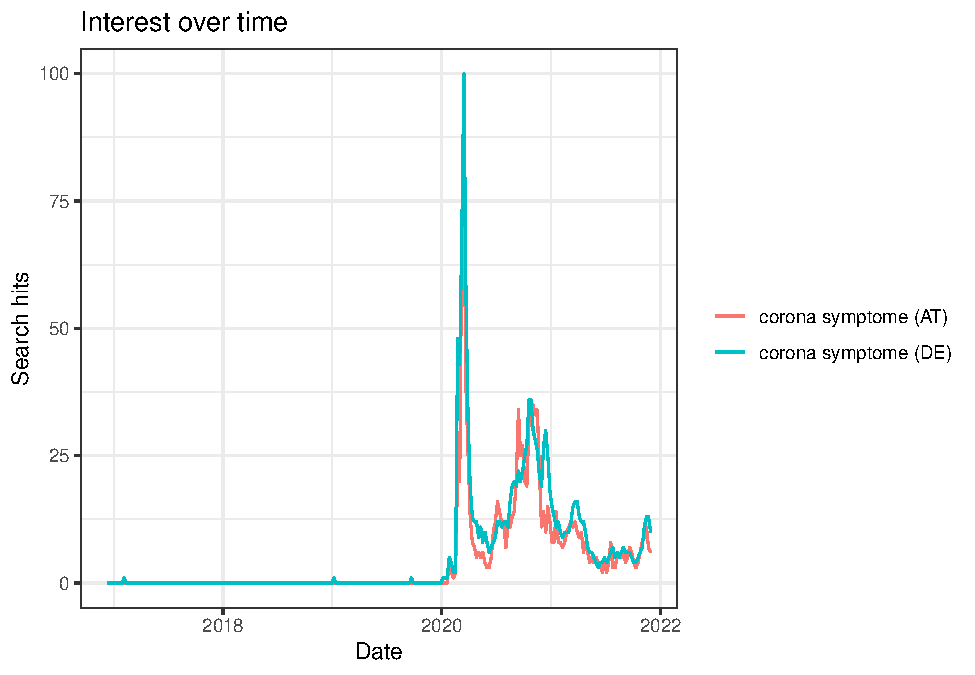
\includegraphics{2021_apis_for_social_scientists_a_collaborative_review_files/figure-latex/unnamed-chunk-49-1.pdf}

\begin{itemize}
\tightlist
\item
  Note (1): the use of c() in the keyword argument of the gtrends function allows comparisons of up to 5 searches (separator = comma).\\
\item
  Note (2): the use of the pattern `\,``xyz''\,' in the keyword argument of the gtrends function corresponds to the inverted commas in the table above, all other punctuation methods in the table above can be used as indicated in the table.
\end{itemize}

\begin{Shaded}
\begin{Highlighting}[]
\CommentTok{\#Combination using dplyr and ggplot}
\NormalTok{trend }\OtherTok{=} \FunctionTok{gtrends}\NormalTok{(}\AttributeTok{keyword=}\StringTok{"corona symptome"}\NormalTok{, }\AttributeTok{geo=}\FunctionTok{c}\NormalTok{(}\StringTok{"DE"}\NormalTok{, }\StringTok{"AT"}\NormalTok{), }\AttributeTok{time =} \StringTok{"2020{-}01{-}01 2021{-}04{-}27"}\NormalTok{, }\AttributeTok{gprop=}\StringTok{"web"}\NormalTok{) }

\NormalTok{trend\_df }\OtherTok{\textless{}{-}}\NormalTok{ trend}\SpecialCharTok{$}\NormalTok{interest\_over\_time}

\NormalTok{trend\_df }\OtherTok{\textless{}{-}}\NormalTok{ trend\_df }\SpecialCharTok{\%\textgreater{}\%}
    \FunctionTok{mutate}\NormalTok{(}\AttributeTok{hits =} \FunctionTok{as.numeric}\NormalTok{(hits), }\AttributeTok{date =} \FunctionTok{as.Date}\NormalTok{(date)) }\SpecialCharTok{\%\textgreater{}\%}
    \FunctionTok{replace}\NormalTok{(}\FunctionTok{is.na}\NormalTok{(.), }\DecValTok{0}\NormalTok{)}

\FunctionTok{ggplot}\NormalTok{(trend\_df, }\FunctionTok{aes}\NormalTok{(}\AttributeTok{x=}\NormalTok{date, }\AttributeTok{y=}\NormalTok{hits, }\AttributeTok{group=}\NormalTok{geo, }\AttributeTok{col=}\NormalTok{geo)) }\SpecialCharTok{+} \FunctionTok{geom\_line}\NormalTok{(}\AttributeTok{size=}\DecValTok{2}\NormalTok{) }\SpecialCharTok{+}
\FunctionTok{scale\_x\_date}\NormalTok{(}\AttributeTok{date\_breaks =} \StringTok{"2 months"}\NormalTok{ , }\AttributeTok{date\_labels =} \StringTok{"\%b{-}\%y"}\NormalTok{) }\SpecialCharTok{+}
\FunctionTok{labs}\NormalTok{(}\AttributeTok{color=} \StringTok{"Countries"}\NormalTok{) }\SpecialCharTok{+}
\FunctionTok{ggtitle}\NormalTok{(}\StringTok{"Frequencies for the query {-}corona symptoms{-} in the period: 01/01/2020 {-} 27/04/2021"}\NormalTok{)}
\end{Highlighting}
\end{Shaded}

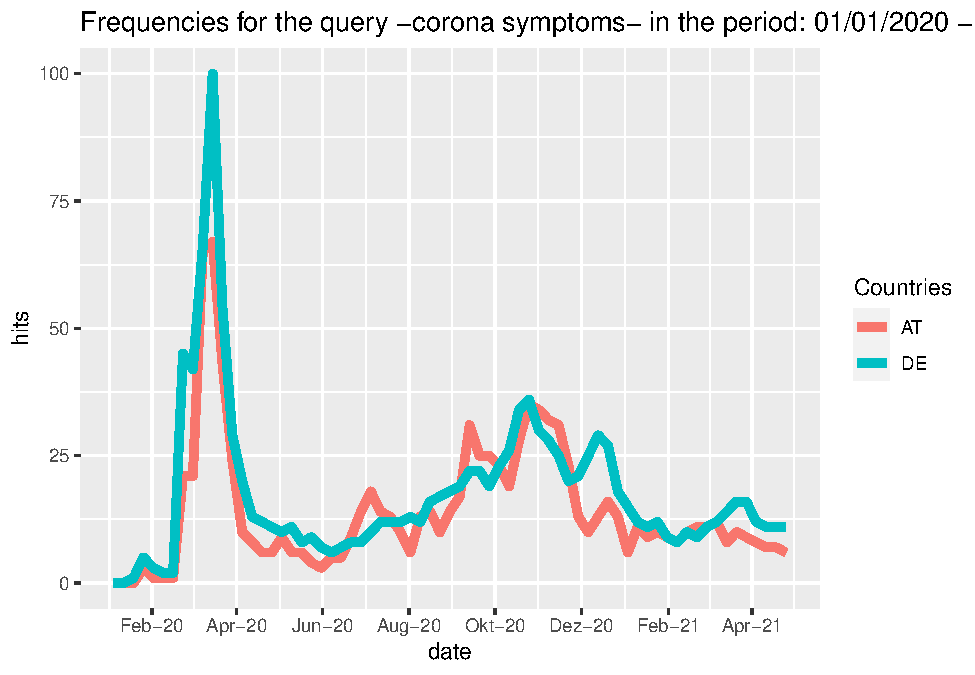
\includegraphics{2021_apis_for_social_scientists_a_collaborative_review_files/figure-latex/unnamed-chunk-50-1.pdf}

\hypertarget{social-science-examples-6}{%
\section{Social science examples}\label{social-science-examples-6}}

\begin{itemize}
\tightlist
\item
  \emph{Are there social science research examples using the API?}
\end{itemize}

Google Trends can be used to predict the outcomes of elections. For example a study by (\citet{Prado-Roman2021}) uses Google Trends data to predict the past four elections in the United States and the past five in Canada, since Google first published its search statistics in 2004. They analysed which candidate had the most Google searches in the months leading up to election day and show, that with the help of this data, all actual winners in all the elections held since 2004 could be predicted.\\
Another example is a study by \citet{Mavragani2019} which uses Google Trends data to predict the results of referendums (Scottish referendum 2014, Greek referendum 2015, British referendum 2016, Hungarian referendum 2016, Italian referendum 2016 and the Turkish referendum 2017). It can be shown that the results from Google Trends data are quite similar to the actual referendum results and in some cases are even more accurate than official polls. It is argued that with the help of Google Trends data revealed preferences instead of users' stated preferences can be analyzed and this data source could be a helpful source to analyze and predict human behavior (given areas where the Internet is widely accessible and not restricted).\\
Furthermore, Google Trends data can also be utilized in other fields, for example to examine whether COVID-19 and the associated lockdowns initiated in Europe and America led to changes in well-being related topic search-terms. The study by \citet{Brodeur2021} finds an increase in queries addressing boredom, loneliness, worry and sadness, and a decrease for search terms like stress, suicide and divorce. Indicating that the people's mental health could have been strongly affected by the pandemic and the lockdowns.

\hypertarget{youtube-api}{%
\chapter{Youtube API}\label{youtube-api}}

Melike Kaplan, Jana Klein

\hypertarget{provided-servicesdata-8}{%
\section{Provided services/data}\label{provided-servicesdata-8}}

\begin{itemize}
\tightlist
\item
  \emph{What data/service is provided by the API?}
\end{itemize}

The API is provided by Google, Youtube's parent company.

There are different types of Youtube APIs that serve different purposes:

\begin{enumerate}
\def\labelenumi{\arabic{enumi}.}
\tightlist
\item
  \textbf{YouTube Analytics API:} retrieves your YouTube Analytics data.
\item
  \textbf{YouTube Data API v3:} provides access to YouTube data, such as videos, playlists, and channels.
\item
  \textbf{YouTube oEmbed API:} \href{https://oembed.com/}{oEmbed} is an elegant way to embed multimedia for a link.
\item
  \textbf{YouTube Reporting API:} Schedules reporting jobs containing your YouTube Analytics data and downloads the resulting bulk data reports in the form of CSV files.
\end{enumerate}

The \href{https://developers.google.com/youtube/v3/sample_requests}{google developer site} provides sample requests and a summary of the possible metrics that the API can give you data on. You can actually run your API requests there. All the possible calls you can make are provided on the page: Captions, ChannelBanners, Channels, ChannelSection, Comments, CommentThreads, i18nLanguages, i18nRegrions, Members, MembershipLevels, Playlistitems, Playlists, Search, Subscriptions, Thumbnails, VideoAbuseReportReasons, VideoCategories, and Videos.

\hypertarget{prerequesites-8}{%
\section{Prerequesites}\label{prerequesites-8}}

\begin{itemize}
\tightlist
\item
  \emph{What are the prerequisites to access the API (authentication)? }
\end{itemize}

First, you will need a Google account which you will use to log into the Google Cloud Platform. You will need to create a new project unless you already have one (\href{https://cloud.google.com/resource-manager/docs/creating-managing-projects}{here you can find more information}). Then, you can search for the four Youtube APIs (YouTube Analytics API, YouTube Data API v3, YouTube oEmbed API, YouTube Reporting API) mentioned above and enable them (\href{https://support.google.com/googleapi/answer/6158841?hl=en}{here you can find more information}).

Then, continue to the ``APIs and Services'' Page from the sidebar and click on ``Credentials.'' Click on ``+ Create Credentials'' at the top of the page. You have three options here: API Key, OAuth client ID or Service account. An API Key will identify your project with a simple key to check quota and access but if you wish to use the YouTube API for your app, you should create an OAuth client ID which will request user consent so that your app can access the user's data. This is also necessary when you want to use the tuber package. A Service account enables server to server, app-level authentication using robot accounts. We will continue with the option of creating an API Key, and later we provide an example of using the OAuth Client ID with the tuber package.

When you click on ``API Key'' in the ``+Create Credentials'' list, a screen will appear like below:

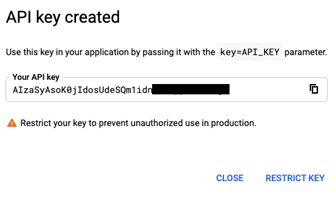
\includegraphics{figures/Image_Youtube_API.png}

Your key is created! It is important to restrict the key!

\hypertarget{simple-api-call-8}{%
\section{Simple API call}\label{simple-api-call-8}}

\begin{itemize}
\tightlist
\item
  \emph{What does a simple API call look like?}
\end{itemize}

The base URL is \url{https://www.googleapis.com/youtube/v3/}.
With the following API call we tried to get the channel statistics from the SWR youtube channel. The channel statistics include information on the viewer count, subscriber count, whether there are hidden subscribers and on the video count.
\url{https://youtube.googleapis.com/youtube/v3/channels?part=statistics\&id=UCy4_zQ59zmS7zO4Dc6vbT_w\&key=\%5BYour_API_Key\%5D}
However, this call did not work for us, we got an error code 400 that said that our API key is not valid.

\hypertarget{api-access-8}{%
\section{API access}\label{api-access-8}}

\begin{itemize}
\tightlist
\item
  \emph{How can we access the API from R (httr + other packages)?}
\end{itemize}

Example to get channel statistics:

\begin{Shaded}
\begin{Highlighting}[]
\FunctionTok{library}\NormalTok{(httr)}
\FunctionTok{library}\NormalTok{(jsonlite)}
\FunctionTok{library}\NormalTok{(here)}
\FunctionTok{library}\NormalTok{(dplyr)}
\FunctionTok{library}\NormalTok{(ggplot2)}
\end{Highlighting}
\end{Shaded}

\begin{Shaded}
\begin{Highlighting}[]
\CommentTok{\#save your API key in the object key}
\NormalTok{key}\OtherTok{\textless{}{-}}\StringTok{"Your\_API\_Key"}

\CommentTok{\#YouTube channels either have a channel id or a user id}
\NormalTok{ZDF\_Magazin\_Royle}\OtherTok{\textless{}{-}}\StringTok{"UCNNEMxGKV1LsKZRt4vaIbvw"} \CommentTok{\#channel id}
\NormalTok{Boilerroom }\OtherTok{\textless{}{-}} \StringTok{"brtvofficial"} \CommentTok{\#user id}

\CommentTok{\#save the base URL in the object base}
\NormalTok{base}\OtherTok{\textless{}{-}} \StringTok{"https://www.googleapis.com/youtube/v3/"}

\CommentTok{\#get channel info with channel id}
\NormalTok{api\_params }\OtherTok{\textless{}{-}} 
  \FunctionTok{paste}\NormalTok{(}\FunctionTok{paste0}\NormalTok{(}\StringTok{"key="}\NormalTok{, key), }
        \FunctionTok{paste0}\NormalTok{(}\StringTok{"id="}\NormalTok{, ZDF\_Magazin\_Royle), }
        \StringTok{"part=snippet,contentDetails,statistics"}\NormalTok{,}
        \AttributeTok{sep =} \StringTok{"\&"}\NormalTok{)}
\NormalTok{api\_call }\OtherTok{\textless{}{-}} \FunctionTok{paste0}\NormalTok{(base, }\StringTok{"channels"}\NormalTok{, }\StringTok{"?"}\NormalTok{, api\_params)}
\NormalTok{api\_result }\OtherTok{\textless{}{-}} \FunctionTok{GET}\NormalTok{(api\_call)}
\NormalTok{json\_result }\OtherTok{\textless{}{-}} \FunctionTok{content}\NormalTok{(api\_result, }\StringTok{"text"}\NormalTok{, }\AttributeTok{encoding=}\StringTok{"UTF{-}8"}\NormalTok{)}

\CommentTok{\#format json into dataframe}
\NormalTok{channel.json }\OtherTok{\textless{}{-}} \FunctionTok{fromJSON}\NormalTok{(json\_result, }\AttributeTok{flatten =}\NormalTok{ T)}
\NormalTok{channel.df }\OtherTok{\textless{}{-}} \FunctionTok{as.data.frame}\NormalTok{(channel.json)}

\CommentTok{\#example with a username}
\NormalTok{api\_params2 }\OtherTok{\textless{}{-}} 
  \FunctionTok{paste}\NormalTok{(}\FunctionTok{paste0}\NormalTok{(}\StringTok{"key="}\NormalTok{, key), }
        \FunctionTok{paste0}\NormalTok{(}\StringTok{"forUsername="}\NormalTok{, Boilerroom), }
        \StringTok{"part=snippet,contentDetails,statistics"}\NormalTok{,}
        \AttributeTok{sep =} \StringTok{"\&"}\NormalTok{)}
\NormalTok{api\_call2 }\OtherTok{\textless{}{-}} \FunctionTok{paste0}\NormalTok{(base, }\StringTok{"channels"}\NormalTok{, }\StringTok{"?"}\NormalTok{, api\_params2)}
\NormalTok{api\_result2 }\OtherTok{\textless{}{-}} \FunctionTok{GET}\NormalTok{(api\_call2)}
\NormalTok{json\_result2 }\OtherTok{\textless{}{-}} \FunctionTok{content}\NormalTok{(api\_result2, }\StringTok{"text"}\NormalTok{, }\AttributeTok{encoding=}\StringTok{"UTF{-}8"}\NormalTok{)}

\CommentTok{\#format json into dataframe}
\NormalTok{channel.json2 }\OtherTok{\textless{}{-}} \FunctionTok{fromJSON}\NormalTok{(json\_result2, }\AttributeTok{flatten =}\NormalTok{ T)}
\NormalTok{channel.df2 }\OtherTok{\textless{}{-}} \FunctionTok{as.data.frame}\NormalTok{(channel.json2)}
\end{Highlighting}
\end{Shaded}

On CRAN we found the \href{https://cran.r-project.org/web/packages/tuber/index.html}{``tuber'' package}. The package enables you to get the comments posted on YouTube videos, number of likes of a video, search for videos with specific content and much more. You can also scrape captions from a few videos. To be able to use the tuber package, not an API key but the authentication with OAuth is necessary. OAuth (Open Authorization) uses authorization tokens to prove an identity between consumers and service providers. You can get your client ID and secret on the Google Cloud Platform under Credentials.

\begin{enumerate}
\def\labelenumi{\arabic{enumi})}
\item
  Setting up the ``Consent Screen''\\
  First we had to configure the so-called OAuth consent screen, where we put ``external'' and then had to put an app name. For scopes we did not specify anything and just clicked save \& continued. To be able to use the API you have to set your own google mail address that you use for the Google cloud.
\item
  Get OAuth credentials\\
  After setting up the consent screen you can go back and click ``create credentials'' and add a ``OAuth client ID''. As a result you get an OAuth client id and secret. You can download this information stored in a JSON file. With the Yt\_oauth function you can then authenticate yourself. This will forward us to logging into our google account. Allow the access to your google account. (like with google bigquery).
\end{enumerate}

\href{https://www.storybench.org/how-to-download-youtube-data-in-r-using-tuber-and-purrr/}{This page} provides some example API calls you can make with the tuber package.

\begin{Shaded}
\begin{Highlighting}[]
\FunctionTok{library}\NormalTok{(tuber) }\CommentTok{\# youtube API}
\FunctionTok{library}\NormalTok{(magrittr) }\CommentTok{\# Pipes \%\textgreater{}\%, \%T\textgreater{}\% and equals(), extract().}
\FunctionTok{library}\NormalTok{(tidyverse) }\CommentTok{\# all tidyverse packages}
\FunctionTok{library}\NormalTok{(purrr) }\CommentTok{\# package for iterating/extracting data}
\end{Highlighting}
\end{Shaded}

\begin{Shaded}
\begin{Highlighting}[]
\CommentTok{\#save client id and secret in an object}
\NormalTok{client\_id}\OtherTok{\textless{}{-}}\StringTok{"put client ID"}
\NormalTok{client\_secret}\OtherTok{\textless{}{-}}\StringTok{"put client secret"}

\CommentTok{\# use the youtube oauth }
\FunctionTok{yt\_oauth}\NormalTok{(}\AttributeTok{app\_id =}\NormalTok{ client\_id,}
         \AttributeTok{app\_secret =}\NormalTok{ client\_secret,}
         \AttributeTok{token =} \StringTok{\textquotesingle{}\textquotesingle{}}\NormalTok{)}

\CommentTok{\#Downloading playlist data}
\CommentTok{\#first get playlist ID}
\NormalTok{go\_psych\_playlist\_id }\OtherTok{\textless{}{-}}\NormalTok{ stringr}\SpecialCharTok{::}\FunctionTok{str\_split}\NormalTok{(}
  \AttributeTok{string =} \StringTok{"https://www.youtube.com/playlist?list=PLD4cyJhQaFwWZ838zZhWVr3RG\_nETlICM"}\NormalTok{, }
  \AttributeTok{pattern =} \StringTok{"="}\NormalTok{, }
  \AttributeTok{n =} \DecValTok{2}\NormalTok{,}
  \AttributeTok{simplify =} \ConstantTok{TRUE}\NormalTok{)[ , }\DecValTok{2}\NormalTok{]}
\NormalTok{go\_psych\_playlist\_id}

\CommentTok{\#use the tuber function get\_playlist\_items to collect the videos into a data frame}

\NormalTok{go\_psych }\OtherTok{\textless{}{-}}\NormalTok{ tuber}\SpecialCharTok{::}\FunctionTok{get\_playlist\_items}\NormalTok{(}\AttributeTok{filter =} 
                                                \FunctionTok{c}\NormalTok{(}\AttributeTok{playlist\_id =} \StringTok{"PLD4cyJhQaFwWZ838zZhWVr3RG\_nETlICM"}\NormalTok{), }
                                              \AttributeTok{part =} \StringTok{"contentDetails"}\NormalTok{,}
                                              \CommentTok{\# set this to the number of videos}
                                              \AttributeTok{max\_results =} \DecValTok{200}\NormalTok{) }

\CommentTok{\# check the data for go Psych}
\CommentTok{\#now we have the video ids of all videos in that playlist}
\NormalTok{go\_psych }\SpecialCharTok{\%\textgreater{}\%}\NormalTok{ dplyr}\SpecialCharTok{::}\FunctionTok{glimpse}\NormalTok{(}\DecValTok{78}\NormalTok{)}
\end{Highlighting}
\end{Shaded}

Package information:\\
* \href{https://cran.r-project.org/web/packages/tuber/index.html}{CRAN - Package tuber}\\
* \href{https://cran.r-project.org/web/packages/tuber/tuber.pdf}{here} you can find all the functions that the tuber package provides

\hypertarget{social-science-examples-7}{%
\section{Social science examples}\label{social-science-examples-7}}

\begin{itemize}
\tightlist
\item
  \emph{Are there social science research examples using the API?}
\end{itemize}

In the study ``Identifying Toxicity Within YouTube Video Comment'' (\citet{Obadimu2019}), the researchers utilized the YouTube Data API to collect the comments from eight YouTube channels that were either pro- or anti NATO. To the comments, five types of toxicity scores were assigned to analyze hateful comments. With word clouds the researchers were able to quantify the count of words from comments. The final dataset contained 1,424 pro-NATO videos with 8,276 comments, and 3,461 anti-NATO videos with 46,464 comments.

The aim of the study ``YouTube channels, uploads and views: A statistical analysis of the past 10 years'' (\citet{Baertl2018}) was to give an overview on how YouTube developed over the past 10 years in terms of consumption and production of videos. The study utilizes a random sample of channel and video data to answer the question. The data is retrieved with the YouTube API (did not specify which one) combined with a tool that generated random string searches to find a near-random sample of channels created between 01.01.2016 and 31.12.2016. Results are that channels, views and video uploads differ according to video genre. Furthermore, the analysis revealed that the majority of views are obtained by only a few channels. On average, older channels have a larger amount of viewers.

In the study ``From ranking algorithms to `ranking cultures': Investigating the modulation of visibility in YouTube search results'' (\citet{Rieder2018}), YouTube is conceptualized as an influential source of information that uses a socio-algorithmic process in order to place search recommendations in a hierarchy. This process of ranking is considered to be a construction of relevance and knowledge in a very large pool of information. Therefore, the search function serves as a curator of recommended content. The information that is being transmitted in this content can also impose certain perspectives on users which is why how the algorithm works is especially important when it comes to controversial issues. In order to better understand how the algorithms that determine search rankings on YouTube work, the authors use a scraping approach and the YouTube API v3 to study the ranking of certain sociocultural issues over time. Examples of the keywords that they use are `gamergate,' `trump,' `refugees' and `syria.' They find three general types of morphologies of rank change.

\hypertarget{ckan-api}{%
\chapter{CKAN API}\label{ckan-api}}

Barbara K. Kreis

The CKAN API is an API offered by the open-source data management system (DMS) CKAN (Open Knowledge Foundation). Currently, CKAN is used as a DMS by many different users, governmental institutions and corporations alike.\\
This API review will focus on the use of the CKAN API to access and work with open government data. As the CKAN DMS is used by various governments to offer open datasets, it is a helpful tool for researchers to access this treasure of publicly open information. CKAN hosts free datasets from various governments, such as from Germany, Canada, Australia, the Switzerland and many more.

\hypertarget{provided-servicesdata-9}{%
\section{Provided services/data}\label{provided-servicesdata-9}}

\begin{itemize}
\tightlist
\item
  \emph{What data/service is provided by the API?}
\end{itemize}

All of CKAN's core features can be accessed via the CKAN API (Open Knowledge Foundation)\\
With the CKAN API, you can

\begin{itemize}
\tightlist
\item
  Get a JSON-formatted list of a site's objects, datasets or groups.
\item
  Get a full JSON representation of an object, e.g.~a dataset.
\item
  Search for any packages (datasets) or resources that match a query.
\item
  Get an activity stream of recently changed datasets on a site.
\end{itemize}

Please see the following \href{https://docs.ckan.org/en/2.8/api/index.html}{link} for more information on the services provided by the CKAN API and some specific examples.\\
When it comes to the specific datasets on the government sites, there are two types that can be accessed: specific datasets and meta data sets.\\
For example, the \href{https://www.govdata.de/impressum}{German} and the \href{https://www.gsa.gov/about-us/organization/federal-acquisition-service/technology-transformation-services}{US Government} have a website each, where you can get access to metadata that include descriptions and URLs about the specific open datasets that can be accessed. These meta datasets can be a starting point for research on a specific topic.\\
The specific datasets include a variety of different contents from public administration, such as election results, data on schools, maps and many more. The German data portal \href{https://www.govdata.de/impressum}{govdata.de} for example serves as a collection point for all those data from various institutions. Those specific administrative institutions are the ones that actually provide the data. Therefore, not every institution provides the same data on the same topic.

\hypertarget{prerequesites-9}{%
\section{Prerequesites}\label{prerequesites-9}}

\begin{itemize}
\tightlist
\item
  \emph{What are the prerequisites to access the API (authentication)? }
\end{itemize}

There are no prerequisites to access the CKAN API. Furthermore, there seem to be no prerequisites to access the open data from the various governmental institutions using CKAN.

\hypertarget{simple-api-call-9}{%
\section{Simple API call}\label{simple-api-call-9}}

\begin{itemize}
\tightlist
\item
  \emph{What does a simple API call look like?}
\end{itemize}

When a user wants to make an API call, two use cases have to be distinguished: Calling meta-data and calling specific datasets.

\emph{Meta-datasets}

When calling the meta data, the DCAT catalog has to be queried. DCAT-AP.de is a German metadata model to exchange open government data. For more information and information on the meta data structure, see this \href{https://www.dcat-ap.de/}{website}.\\
The API call for the DCAT catalog can deliver three formats: RDF, Turtle and JSON-LD. The type of format can be specified at the end of the request (e.g.~``format=jsonld'').\\
The following API call is an example for the search term ``Kinder''.
\url{https://ckan.govdata.de/api/3/action/dcat_catalog_search?q=kinder\&format=jsonld}

\emph{Specific datasets from GovData}

To look for specific datasets, not the meta data, only little has to be changed in the URL. In the case of querying specific datasets, the response format is JSON.
The following API call is an example when looking for the first 5 packages (datasets) that contain the search term ``Kinder'' (=children).\\
\url{https://www.govdata.de/ckan/api/3/action/resource_show?q=kinder}

\hypertarget{api-access-9}{%
\section{API access}\label{api-access-9}}

\begin{itemize}
\tightlist
\item
  \emph{How can we access the API from R (httr + other packages)?}
\end{itemize}

The CKAN API can be accessed from R with the \href{https://cran.r-project.org/web/packages/httr/vignettes/quickstart.html}{httr package} or the \href{https://cran.r-project.org/web/packages/ckanr/ckanr.pdf}{ckanr package}.\\
Please note that as a scientist you can only use GET requests. All kinds of POST requests are restricted to government employees that work at the institutions which provide the data sets.

\begin{Shaded}
\begin{Highlighting}[]
\CommentTok{\# CKAN API \#}
\CommentTok{\# Option 1: Use the httr package to access the API}

\FunctionTok{library}\NormalTok{(httr) }\CommentTok{\# required to work with the API}

\CommentTok{\# With the following query we get the same information as described in the paragraph above}

\NormalTok{base\_url }\OtherTok{\textless{}{-}} \StringTok{"https://www.govdata.de/ckan/api/3/action/resource\_show"}
\NormalTok{berlin }\OtherTok{\textless{}{-}} \FunctionTok{GET}\NormalTok{(base\_url, }\AttributeTok{query=}\FunctionTok{list}\NormalTok{(}\AttributeTok{q=}\StringTok{"kinder"}\NormalTok{,}\AttributeTok{rows=}\DecValTok{5}\NormalTok{))}
\end{Highlighting}
\end{Shaded}

\begin{Shaded}
\begin{Highlighting}[]
\CommentTok{\# Option 2: Use the ckanr package to access the API}

\CommentTok{\# load relevant packages}
\FunctionTok{library}\NormalTok{(tidyverse)}
\FunctionTok{library}\NormalTok{(ckanr)}
\FunctionTok{library}\NormalTok{(jsonlite)}
\FunctionTok{library}\NormalTok{(readxl)}
\FunctionTok{library}\NormalTok{(curl)}
\FunctionTok{library}\NormalTok{(readxl)}

\CommentTok{\#connect to the website}
\NormalTok{url\_site }\OtherTok{\textless{}{-}} \StringTok{"https://www.govdata.de/ckan"}
\FunctionTok{ckanr\_setup}\NormalTok{(}\AttributeTok{url =}\NormalTok{ url\_site)}

\CommentTok{\# first, let\textquotesingle{}s see which groups are on this site}
\FunctionTok{group\_list}\NormalTok{(}\AttributeTok{as =} \StringTok{"table"}\NormalTok{)}


\CommentTok{\#you can see there are different groups}
\CommentTok{\#now we want to look at them in more detail}
\FunctionTok{group\_list}\NormalTok{(}\AttributeTok{limit =} \DecValTok{2}\NormalTok{)}

\CommentTok{\# now you can look for the specific packages}
\FunctionTok{package\_list}\NormalTok{(}\AttributeTok{as =} \StringTok{"table"}\NormalTok{)}

\CommentTok{\# now, let\textquotesingle{}s look at a specific package more closely, to get some more information}
\FunctionTok{package\_show}\NormalTok{(}\StringTok{"100{-}jahre{-}stadtgrun{-}stadtpark{-}und{-}volkspark"}\NormalTok{)}

\CommentTok{\# now, let\textquotesingle{}s do a more specific search for specific resources (we look at Kinder = kids/ children)}
\NormalTok{x }\OtherTok{\textless{}{-}} \FunctionTok{resource\_search}\NormalTok{(}\AttributeTok{q =} \StringTok{"name:Kinder"}\NormalTok{, }\AttributeTok{limit =} \DecValTok{3}\NormalTok{)}
\NormalTok{x}\SpecialCharTok{$}\NormalTok{results}

\CommentTok{\# here you get the name, the Description (not always filled out) and the data format}

\CommentTok{\# now we want to have a closer look at the second resource (day care for children)}
\CommentTok{\# we need to get the url, by using the resource number}

\NormalTok{url}\OtherTok{\textless{}{-}}\FunctionTok{resource\_show}\NormalTok{(}\AttributeTok{id =}\StringTok{"a8413550{-}bf4d{-}40f3{-}921a{-}941da3fce132"}\NormalTok{)}
\NormalTok{url}\SpecialCharTok{$}\NormalTok{url}

\CommentTok{\# with the url, we can now import the data}
\NormalTok{url }\OtherTok{\textless{}{-}}\NormalTok{ (}\StringTok{"https://geo.sv.rostock.de/download/opendata/kindertagespflegeeinrichtungen/kindertagespflegeeinrichtungen.csv"}\NormalTok{)}
\NormalTok{destfile }\OtherTok{\textless{}{-}}\NormalTok{ (}\StringTok{"kindertagespflegeeinrichtungen.csv"}\NormalTok{)}
\NormalTok{curl}\SpecialCharTok{::}\FunctionTok{curl\_download}\NormalTok{(url, destfile)}

\NormalTok{kindertagespflegeeinrichtungen }\OtherTok{\textless{}{-}} \FunctionTok{read\_csv}\NormalTok{(destfile)}
\FunctionTok{View}\NormalTok{(kindertagespflegeeinrichtungen)}

\CommentTok{\# in this file, you can now for example look at the opening hours of the day cares in Rostock (a German city)}
\end{Highlighting}
\end{Shaded}

\hypertarget{social-science-examples-8}{%
\section{Social science examples}\label{social-science-examples-8}}

\begin{itemize}
\tightlist
\item
  \emph{Are there social science research examples using the API?}
\end{itemize}

When looking for social science research that used the CKAN API and Open Government data (OGD), it seems that there is more papers and research on the usage of those data, than on the data themselves (\citet{Bedini2014}, \citet{Correa2015}).
In a recent paper that examines the use of OGD (\citet{Quarati2019-jf}), the authors come to the conclusion, that on the one hand many OGD portals lack information about data usage, and on the other hand, where those information can be found, it becomes obvious that the data are only rarely used.\\
For example, regarding the German OGD portal ``GovData.de'', I did not find any social science papers that specifically used data from GovData.de. However, there are a few papers available that describe the German open data initiative (\citet{Liu2018}) and the metadata (\citet{Marienfeld2013}) that can be found on GovData.de.

\hypertarget{mediawiki-action-api}{%
\chapter{MediaWiki Action API}\label{mediawiki-action-api}}

Noam Himmelrath, Jacopo Gambato

\hypertarget{provided-servicesdata-10}{%
\section{Provided services/data}\label{provided-servicesdata-10}}

\begin{itemize}
\tightlist
\item
  \emph{What data/service is provided by the API?}
  To access \emph{Wikipedia}, \emph{MediaWiki} provides the MediaWiki Action API.
\end{itemize}

The API can be used for multiple things, such as accessing wiki features, interacting with a wiki and obtaining meta-information about wikis and public users. Additionally, the web service can provide access data and post changes of \emph{Wikipedia}-webpages.

\hypertarget{prerequesites-10}{%
\section{Prerequesites}\label{prerequesites-10}}

\begin{itemize}
\tightlist
\item
  \emph{What are the prerequisites to access the API (authentication)? }
\end{itemize}

No pre-registration is required to access the API. However, for certain actions, such as very large queries, a registration is required. Moreover, while there is no hard and fast limit on read requests, the system administrators heavily recommend limiting the request rate to secure the stability of the side. It is also best practice to set a descriptive User Agent header.

\hypertarget{simple-api-call-10}{%
\section{Simple API call}\label{simple-api-call-10}}

\begin{itemize}
\tightlist
\item
  \emph{What does a simple API call look like?}
\end{itemize}

As mentioned, the API can be used to communicate with Wikipedia for a variety of actions. As it is most likely for social scientist to extract information rather than post changes to a Wikipedia page, we focus here on obtaining from Wikipedia the information we need.

We include a basic API call to obtain information about the Albert Einstein Wikipedia page

\texttt{https://en.wikipedia.org/w/api.php?action=query\&format=json\&prop=info\&titles=Albert\%20Einstein}

to be plugged into the search bar of a browser to obtain the basic information on the page.

Notice that the first line is common for all calls of the API, while the second line relates to the specific action you are trying to perform.

\hypertarget{api-access-10}{%
\section{API access}\label{api-access-10}}

\begin{itemize}
\tightlist
\item
  \emph{How can we access the API from R (httr + other packages)?}
\end{itemize}

The most common tool is \texttt{WikipediR}, a wrapper around the Wikipedia API. It allows \texttt{R} to access information and ``directions'' for the relevant page or pages of Wikipedia and the content or metadata therein. Importantly, the wrapper only allows to gather information, which implies that the instrument needs to be accompanied by other packages such as \texttt{rvest} for scraping and \texttt{XML} or \texttt{jsonlite} for parsing.

We report here the code to obtain the same information as in the previous example through \texttt{R}:

\begin{Shaded}
\begin{Highlighting}[]
\NormalTok{WikipediR}\SpecialCharTok{::}\FunctionTok{page\_info}\NormalTok{(}
    \AttributeTok{language =} \StringTok{"en"}\NormalTok{, }
    \AttributeTok{project =} \StringTok{"wikipedia"}\NormalTok{, }
    \AttributeTok{page =} \StringTok{"Albert Einstein"}\NormalTok{, }
    \AttributeTok{properties =} \StringTok{"url"}\NormalTok{)}
\end{Highlighting}
\end{Shaded}

\begin{verbatim}
## $batchcomplete
## [1] ""
## 
## $query
## $query$pages
## $query$pages$`736`
## $query$pages$`736`$pageid
## [1] 736
## 
## $query$pages$`736`$ns
## [1] 0
## 
## $query$pages$`736`$title
## [1] "Albert Einstein"
## 
## $query$pages$`736`$contentmodel
## [1] "wikitext"
## 
## $query$pages$`736`$pagelanguage
## [1] "en"
## 
## $query$pages$`736`$pagelanguagehtmlcode
## [1] "en"
## 
## $query$pages$`736`$pagelanguagedir
## [1] "ltr"
## 
## $query$pages$`736`$touched
## [1] "2021-12-05T18:46:13Z"
## 
## $query$pages$`736`$lastrevid
## [1] 1058773374
## 
## $query$pages$`736`$length
## [1] 183211
## 
## $query$pages$`736`$fullurl
## [1] "https://en.wikipedia.org/wiki/Albert_Einstein"
## 
## $query$pages$`736`$editurl
## [1] "https://en.wikipedia.org/w/index.php?title=Albert_Einstein&action=edit"
## 
## $query$pages$`736`$canonicalurl
## [1] "https://en.wikipedia.org/wiki/Albert_Einstein"
## 
## 
## 
## 
## attr(,"class")
## [1] "pageinfo"
\end{verbatim}

\hypertarget{social-science-examples-9}{%
\section{Social science examples}\label{social-science-examples-9}}

\begin{itemize}
\tightlist
\item
  \emph{Are there social science research examples using the API?}
\end{itemize}

Some papers using Wikipedia-information rely on the API to access the data. These papers cover a wide range of social and economical sciences. Political science papers are, for example, concerned with political elections, more specifically election prediction \citep{margolin2016wiki, salem2021wikipedia}. Other papers use the data accessed through the API to analyze media coverage of the COVID-19 pandemic \citep{gozzi2020collective} or the interplay between online information and investment markets \citep{elbahrawy2019wikipedia}.

\hypertarget{references}{%
\chapter{References}\label{references}}

\end{document}
